

\chapter{Elastic Moduli, Oxidation and Load-Partitioning Tests}

\section{Elastic Moduli Measurements Using RUS}

Resonant Ultrasound Spectroscopy (RUS) is a niche technique that is used in the Earth Sciences to determine various elastic moduli across a wide of temperatures.  It can experimentally measure the resonant frequencies of the vibrational modes of an elastic specimen that has stress-free boundary conditions (Figure \ref{fig:rus_elastic}) ~\cite{maynard92}.  Anelastic mechanisms during phase transformations have been explored using this method ~\cite{zhang10}.  The dependence of elastic properties through a phase transition on grain size have also been explored using this method ~\cite{carpenter06, mcknight08, mcknight09}.  This technique has not been used to evaluate the elastic properties of nickel-based superalloys and silicides.

In a bullk isotropic polycrystalline material, there are two independent bulk elastic constants:  bulk modulus, K, and shear modulus, G.  There are more independent elastic constants for single crystal specimens.  In this study, polycrystalline specimens that had the smallest extent of anisotropy were used.  These were manufactured by the plasma-melt process.  Polycrystalline material manufactured by the DS process were not used due to their bulk anisotropy.

When tested with RUS, specimens that have substantial micro-cracks would substantially dissipate ultrasound, as identified by peak broadening.  This occurs because of an acoustic loss that accompanies the movement of a crack when a stress is applied.  Specimens that contain a large crack would not dissipate ultrasound to the same extent.  If a crack does not move in the timescale of the applied stress, no dissipation would be observed.  Sharp peaks can still be obtained from such specimens.  There may be specimens containing cracks that do not change  acoustic properties, but such specimens are rare.  

This is an easy non-destructive method for qualitatitive evaluation of specimen quality.  Specimens that have large cracks do not survive machining due to the materials' brittle nature.  Specimens that have micro-cracks may survive manufacture, but these cracks would result in the ultrasound dissipation and can be easily identified.

%
\begin{figure}[H]
\begin{center}
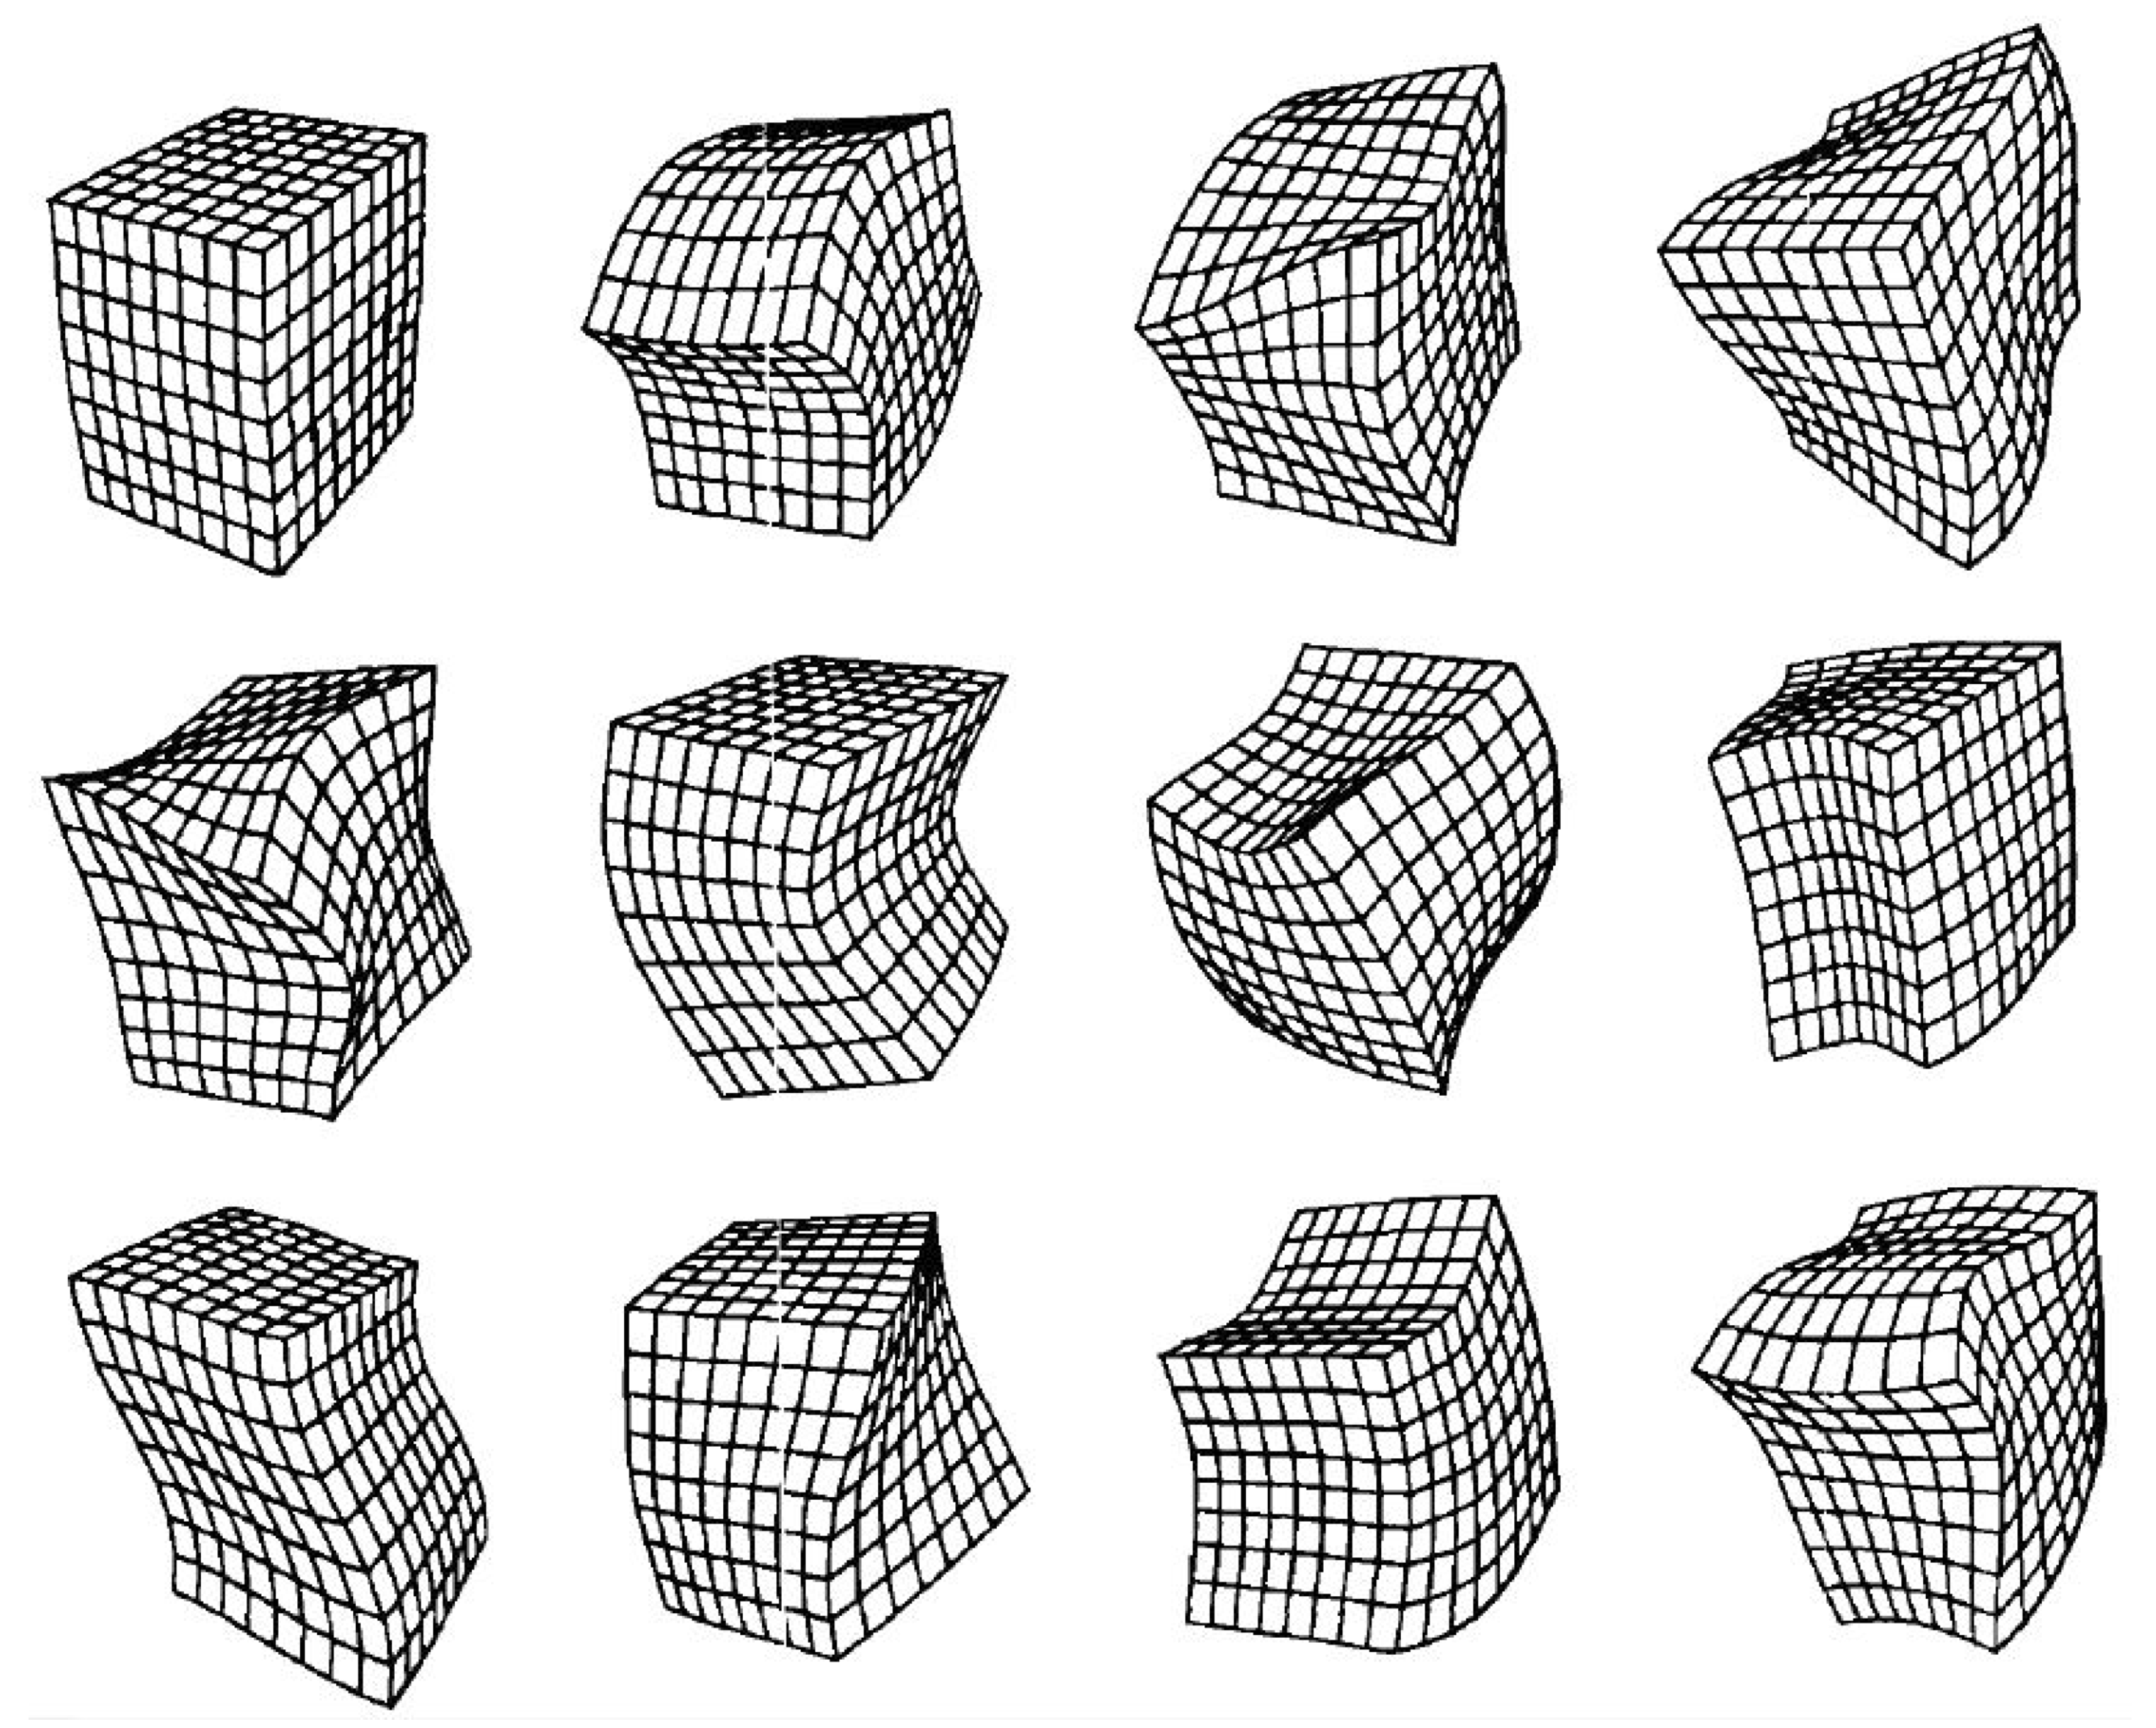
\includegraphics[width=9cm]{rus_elastic}
\caption{Schematic representation of some of the normal modes of vibration of an elastic cube with stree-free boundary conditions ~\cite{maynard92}.}
\label{fig:rus_elastic}
\end{center}
\end{figure}
%

\subsubsection{RUS Experimental Set-up}

The parallelpiped sample is positioned with diametrically opposite corners lightly held by the transducers (Figure \ref{fig:rus_setup}).  In doing so, all normal modes of specimen vibration would be active, and no resonances will be missed.  A frequency synthesizer drives a transducer across a range of ultrasonic frequencies (0.1--2MHz), in small increments, at a constant amplitude.  The other transducer detects displacement induced by specimen vibration, and this displacement is the output of the test.  The output peak profiles are then fitted to produce experimentally determined elastic constants.  


%
\begin{figure}[H]
\begin{center}
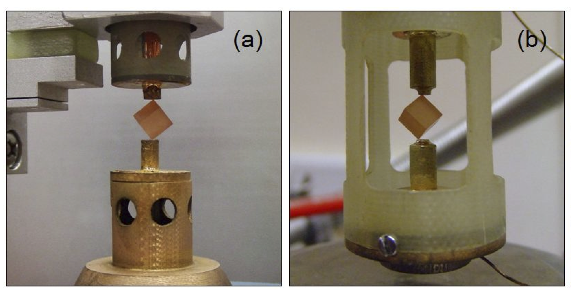
\includegraphics[width=12cm]{rus_setup}
\caption{Photographs of the loaded specimen chamber ~\cite{mcknight09}.}
\label{fig:rus_setup}
\end{center}
\end{figure}
%

Good peak fit can be achieved if the following conditions are met:
\begin{enumerate}
\item test specimens are homogeneous and free of flaws and impurities
\item test specimens must have a very low degree of geometrical error

\item measured resonances have to be correctly assigned to modes during peak fitting
\item to avoid reaching a local minimum during peak fitting, the initial guesses of elastic constants have to be close to actual values 
\item the number of missed modes cannot exceed 10\% of the total number of measured frequencies
\end{enumerate}

High-temperature RUS tests have been succesfully performed on other materials ~\cite{mcknight09}.  Such tests are performed in an open-air furnace.  Although high-temperature elastic constants would be more pertinent than ambient temperature measurements, they could not be acquired as there was no furnace with an inert atmosphere suitable for this experimental set-up.  Only room temperature data was acquired in this project.


\subsubsection{Sample Manufacture}

Sample preparation is the most critical step in this form of testing.  Samples must be polycrystalline and isotropic in order to get all possible elastic constants.  Different code is used to fit the peak profiles of parallelpipeds and cylinders.  Parallelpipeds are easier to fit because of the familiarity the group has with fitting the obtained data.  Cubic crystal structures are an easy class of material to fit.  The peak profiles produced are more distinct, and acquisition of good data is easier.

Rectangular parallelpiped samples were cut from the PM manufactured ingots using an EDS machine that was lubricated with deionised water.  Due to many cracks being present in the ingots, and the intrinsic brittle nature of the alloys, quality specimens were manufactured with difficulty.  Attempts at cutting specimens with a diamond saw resulted in the diamond saw getting worn down.  This difficulty in sample cutting has been encountered in other intermetallics such as ErCo$_2$ and NdCo$_2$.  


Cylinders and parallelpipeds of adequate quality could not be manufactured out of PM-manufactured Cr--Cr$_3$Si.  The intrinsic poor fracture-toughness of the alloy, together with micro-cracks and residual cooling stresses led to crumble-prone material.  Adequate data could not be collected to estimate its Young's Modulus.  No ingot of any ternary alloys were manufactured with the PM process, and these alloys were not tested.  In the end, only the binary alloy V--V$_3$Si, the quaternary alloy \ilovewill{山}Ta, and the quinary alloy \ilovewill{山}TaAl were tested.  

The parallelpipeds used for RUS measurements were slightly larger than the sizes usually used, with dimensions of about 3.00 by 4.00 by 5.00\milli\meter\ and masses of 0.35-0.46 \gram\ (Table \ref{tab:RT}).  Care was taken to ensure that specimen height, width and breadth were different.  With such non-cubic specimens, resonance peaks become more widely distributed.  This increases the ease of subsequent peak-fitting.  Specimen masses were measured to 4 decimal places using an electronic analytical balance.  The alloy densities determined from these parameters, when compared to their theoretical densities (Table \ref{tab:alloycompowt}), are about 100\% for V--V$_3$Si (5.78 \gram\usk\centi\rpcubic\metre), and about 80\% for \ilovewill{山}Ta (9.47 \gram\usk\centi\rpcubic\metre) and \ilovewill{山}TaAl (9.14 \gram\usk\centi\rpcubic\metre).  This is consistent with the observation noted earlier that regions of \ilovewill{山}TaAl had virtually no Ta content.

The large differences of 20\%  between theoretical and measured densities are probably due to a low Ta content in \ilovewill{山}Ta and \ilovewill{山}TaAl stemming from ingot segregation.  These measured densities are also higher than the calculated density of \ilovewill{山} (6.3 \gram\usk\centi\rpcubic\metre), and so both specimens contain some level of Ta.  These specimens, being manufactured by the PM process, should be fully dense.

%
\begin{table}[htdp]
\begin{center}
\begin{tabular}{lccccc}
\hline
\hline
Alloy				&	Manufacture Method&Dimensions (\milli\rpcubic\meter) 	& Mass (g)	& Density(g \centi\rpcubic\meter) \\
\hline

V--V$_3$Si 		&	Plasma-melt	&		2.974 x 3.980 x 5.013			&		0.3470	&		5.848\\

\ilovewill{山}Ta 	&	Plasma-melt	&		2.976 x 3.976 x 5.151			&		0.4614&		7.570\\

\ilovewill{山}TaAl 	&	Plasma-melt	&		2.977 x 3.982 x 5.011			&		0.4271&		7.190\\

\hline
\hline
\end{tabular}
\end{center}
\caption{Physical properties of specimens tested with RUS at room temperature.}
\label{tab:RT}
\end{table}

\subsubsection{Peaks Acquired}
%
The peak profiles for the binary alloy V--V$_3$Si, the quaternary alloy \ilovewill{山}Ta, and the quinary alloy \ilovewill{山}TaAl were acquired.  The peaks obtained from V--V$_3$Si were the sharpest (Figure \ref{fig:rus_v_pm}).  These sharp peaks would have highest chance of a successful fit.  Those from \ilovewill{山}TaAl were the broadest (Figure \ref{fig:rus_santa_pm} and \ref{fig:rus_santaal_pm}).  This is probably due to sample cracks or some other reason for acoustic defect dissipation.  It was surprising that \ilovewill{山}Ta (Figure \ref{fig:rus_santa_pm}) had sharper resonance peaks than \ilovewill{山}TaAl (Figure \ref{fig:rus_santaal_pm}), as the microstructure of \ilovewill{山}Ta is less homogeneous than \ilovewill{山}TaAl, with partially melted pieces of Ta scattered throughout.  Perhaps the \ilovewill{山}Ta sample measured did not have a high Ta content due to segregation.  After all, a couple of specimens had crumbled during machining; the result for \ilovewill{山}Ta could be skewed towards a higher value than the actual value.  When peak profiles of other specimens were acquired for these alloys, the data looked reproducible. 

%
\begin{figure}[H]
\begin{center}
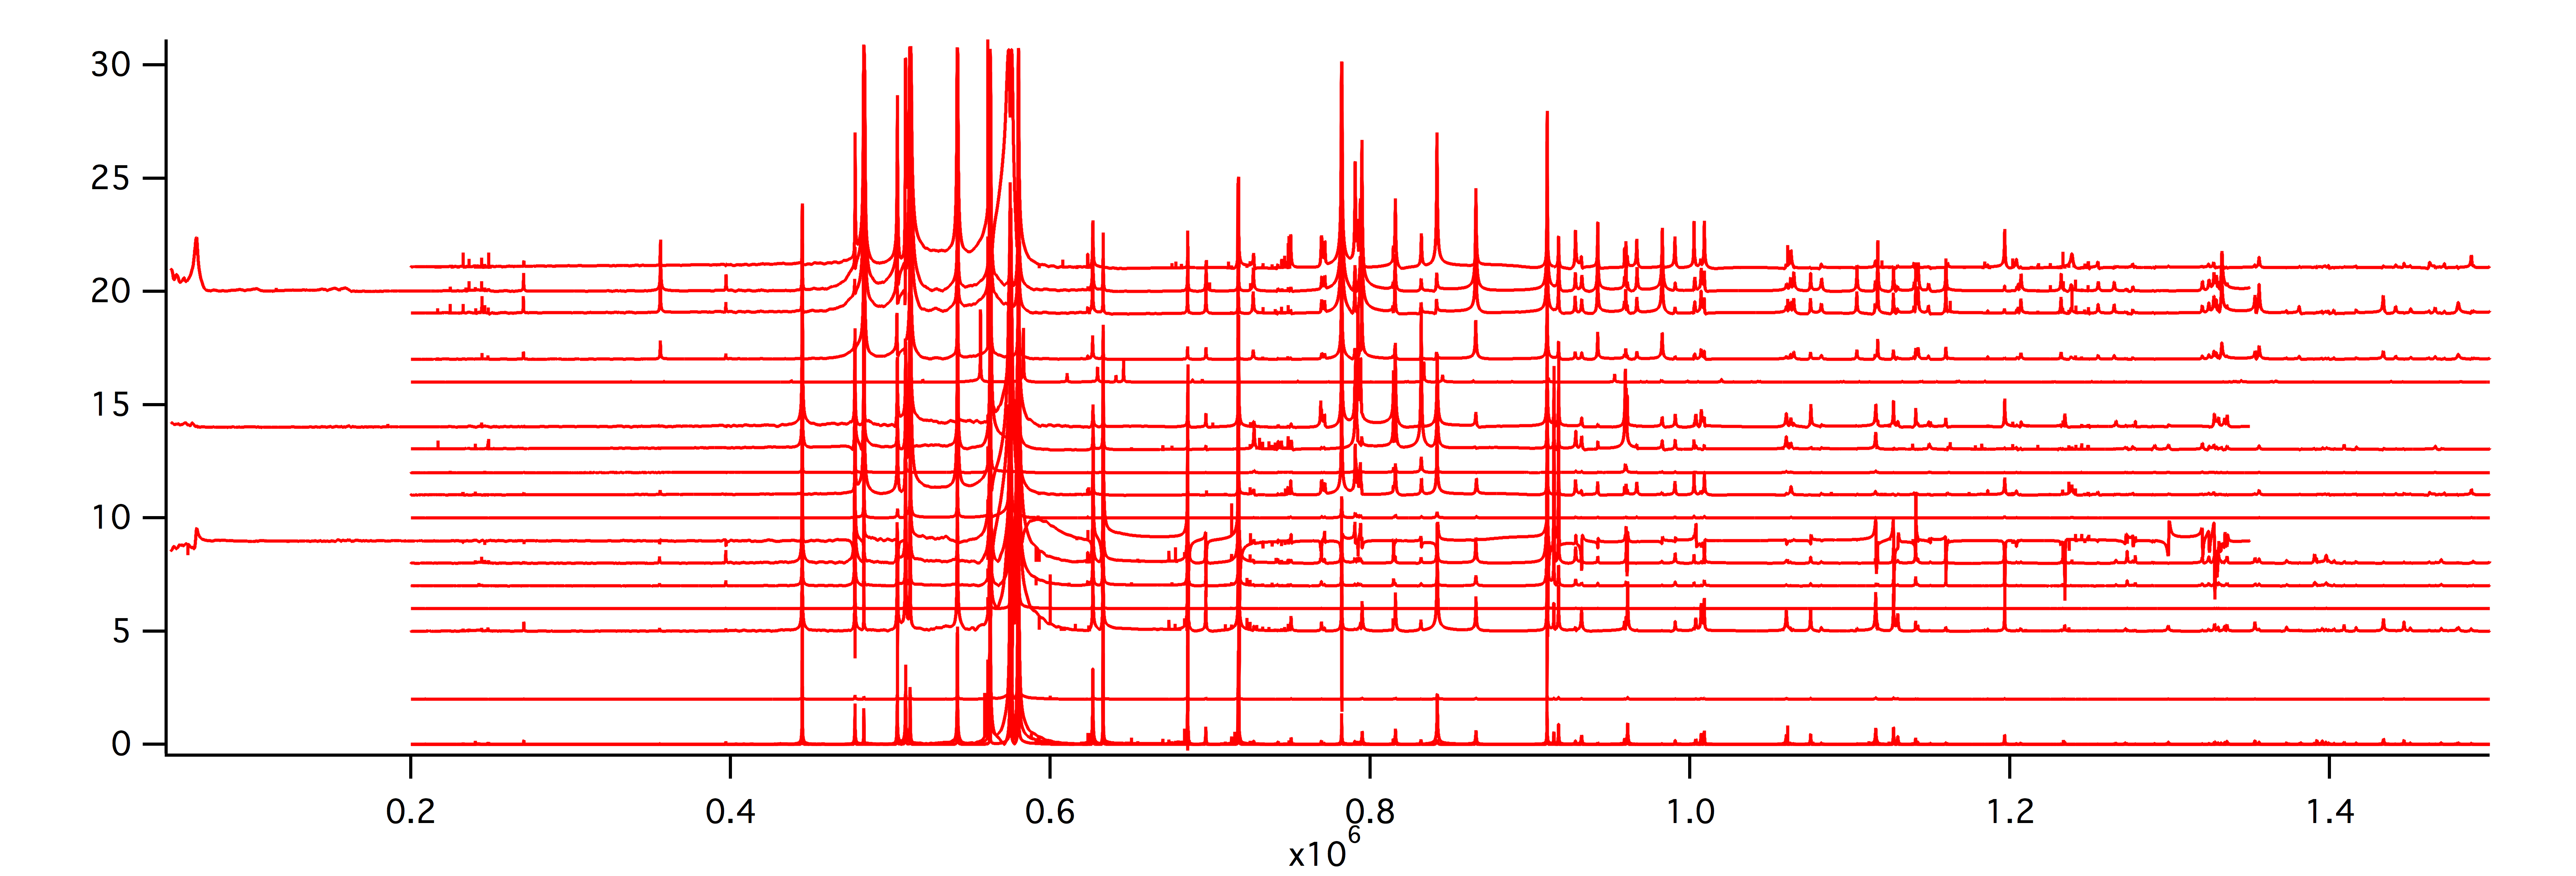
\includegraphics[width=17cm]{RUS_v_pm}
\caption{Peaks obtained for a PM manufactured V--V$_3$Si specimen at all possible orientations of a parallelpiped.}
\label{fig:rus_v_pm}
\end{center}
\end{figure}
%


%
\begin{figure}[H]
\begin{center}
\includegraphics[width=16cm]{RUS_santa_pm}
\caption{Peaks obtained for a PM manufactured \ilovewill{山}Ta specimen at all possible orientations of a parallelpiped.}
\label{fig:rus_santa_pm}
\end{center}
\end{figure}
%


%
\begin{figure}[H]
\begin{center}
\includegraphics[width=16cm]{RUS_santaal_pm}
\caption{Peaks obtained for a PM manufactured \ilovewill{山}TaAl specimen at all possible orientations of a parallelpiped.}
\label{fig:rus_santaal_pm}
\end{center}
\end{figure}
%



\subsubsection{Peak Fitting Procedure}

RUS is a technique that is not commonly used, and the databases available exist for a narrow range of material.  Unsurprisingly, there are no available databases on the alloy systems studied in this work.  If there are missing peaks that cannot be acquired due to anisotropic specimens, the position of these missing peaks cannot be determined, and satisfactory fit may not be achieved.  In order to ensure that all peaks that can be acquired from all elastic constants, data should be collected from all possible specimen configurations between the test chamber grips.  There are five such configurations: three corner configurations, two edge configurations and one face configurations with the long edge upright.

If the peak profile collected is made up of only elastic peaks, it would be very easy to obtain an accurate fit.  High specimen dissipation will result in broad peaks of low intensity.  It would be difficult to obtain robust fits for such peak profiles.  During peak-fitting, broad and small peaks may be omitted if doing so improves fit.  Such peaks may be due to noise.  Sharp and strong peaks should not be omitted, as this would introduce a skew in the data-set.  

Good data that has been fitted well would have an root mean square (rms) error, the error for the whole fit, of less than 0.3\%, for a peak profile with 25 fitted peaks.  28 peaks in the peak profile of V--V$_3$Si were fitted with an rms error of 0.4\%.  This is still considered a robust fit.  Measured values of bulk moduli and shear moduli can be found in Table \ref{tab:young}.  

%
\begin{table}[htdp]
\begin{center}
\begin{tabular}{lccccccc}
\hline
\hline
Alloy&Peak Fitted& K (GPa)& G (GPa)&v& E (GPa)&rms error (\%)	\\	
\hline
V--V$_3$Si	&28 peaks&144.4$\pm$2.2		&58.4$\pm$0.07		&0.32	&154.3		&0.39				\\			
\ilovewill{山}Ta&23 peaks&144.2$\pm$1.8		&91.4$\pm$0.18		&0.24	&226.4		&0.61				\\			
\ilovewill{山}TaAl&14 peaks&87.9$\pm$1.1		&84.7$\pm$0.32		&0.14	&192.3		&1.04				\\			
\hline
\hline
\end{tabular}
\end{center}
\caption{Elastic properties of specimens tested with RUS at room temperature, where K is bulk modulus, G is shear modulus, v is Poisson's ratio, E is Young's Modulus and rms error is root mean square error.}
\label{tab:young}
\end{table}

\vspace{0.5cm}
Young's modulus can be calculated from the measured values of bulk and shear moduli, as it is a function of these moduli and Poisson's ratio:

\hspace{5cm}				$G = \frac{E}{2(1+v)}$

\hspace{5cm}				$K = \frac{E}{3(1-2v)}$

The calculated Young' modulus values have been put in Table \ref{tab:young}.

The peak profile for V--V$_3$Si fitted very well, and produced measured values of 144.4GPa for bulk modulus, and 58.4GPa for shear modulus  (Table \ref{tab:young}).  Young's modulus was calculated to be 154.3GPa from these values.  These are very high values.  The peak profile for \ilovewill{山}Ta was fitted less well, but can still be considered a sound fit, with an rms of 0.61\%.  \ilovewill{山}Ta had a bulk modulus identical to V--V$_3$Si, and a higher shear modulus of 91.4GPa.  Its calculated Young's modulus is 226.4GPa.  

A reasonable shear modulus was found for \ilovewill{山}TaAl, but with poorer accuracy than those for V--V$_3$Si and \ilovewill{山}Ta, with an rms error ($\chi$$^2$) of over 1\% (Table \ref{tab:young}).  A $\chi$$^2$ value of 2 for bulk modulus would typically be considered good data, but the $\chi$$^2$ values for room temperature data of \ilovewill{山}TaAl and \ilovewill{山}Ta were more than 2 for both alloys.  However, since shear is tightly constrained, despite the poor peak fits achieved for \ilovewill{山}TaAl, this shear modulus value of 84.7GPa can be considered sound.  The magnitude of the first large peak occurring at a low frequency is dominated by the shear modulus.  If this peak can be fitted well, one can obtain a reasonably accurate value of shear modulus.  Bulk modulus is not as tightly constrained, and no robust value was found for \ilovewill{山}TaAl.  Although its exact value is unknown, the Young's modulus of \ilovewill{山}TaAl is higher than V--V$_3$Si and lower than \ilovewill{山}Ta.

The fitting error values calculated by the peak-fitting program do not scale linearly. With less accurate moduli and elastic constant values, their corresponding percentage errors cannot be estimated accurately.  Nonetheless, these values have been placed in Table \ref{tab:young} to enable qualitative comparison.

Peak profiles acquired from specimens of directionally solidification manufactured \ilovewill{山} and \ilovewill{山}TaAl showed low dissipation.  This indicates that residual stresses that stem from the differential in coefficients of thermal expansion cooling were not substantial enough to form micro-cracks.  These profiles could not be fitted as there were several peaks missing due to material anisotropy.


\section{Oxidation Tests}

In the initial stages of alloy design, a cursory examination of alloy oxidation properties would be sufficient to determine the alloy suitability for high-temperature applications.  If these properties are poor, excellent oxidation resistance would be inconsequential.  It is not difficult to improve an alloy’s oxidation resistance; however, improving oxidation resistance without substantially compromising an alloy’s high-temperature properties is a non-trivial matter.  Since an alloy's high-temperature mechanical properties are more pertinent, in-depth oxidation studies would be more relevant in the intermediate or final stages of alloy development.  In addition, it was difficult to conduct oxidation tests on these alloys.  For instance, a thermo-gravimetric study of the ternary, quaternary and quinary alloys were considered.  During high-temperature exposure, these alloys would emit vanadium pentoxide as a volatile by-product.  This will condense upon any cool interior surfaces of the thermo-gravimetric analysis (TGA) apparatus. Vanadium pentoxide is known to react with the protective aluminium oxide formed by superalloys and cause substantial premature oxide spallation, even when present in very small amounts.  It is also a health hazard.  Since the in-house TGA apparatus is mostly used for evaluating alumina-forming superalloys, it was deemed best not to sully the interior walls of the apparatus for the sake of collecting preliminary oxidation data of these eutectic alloys. 

To ascertain the limit of vanadium substitution for chromium prior to runaway oxidation, five alloys within the tie-tetrahedron of the (Cr, V)--(Cr, V)$_3$Si system have been investigated following 10-hour isothermal exposures at 800\celsius\ and 1200\celsius.   All specimens were polished to a mirror finish, placed in alumina crucibles and into a box furnace at their respective temperatures, then air-cooled at the end of 10 hours.

At 800\celsius, the Cr--Cr$_3$Si eutectic performs well, forming a green chromia layer (Figure:\ref{fig:oxidation}a).  At 1200\celsius, most of its oxide spalls off upon cooling, as there was insufficient Si content in the alloy to form a protective SiO$_2$ layer (Figure:\ref{fig:oxidation}b).  Chromium oxide is a dense adherent oxide of choice for temperatures below 950\celsius, but is reported to be volatile above it [19]. 
Rust-coloured, oxygen permeable V$_2$O$_5$ has resulted in runaway oxidation in the V--V$_3$Si eutectic at both temperatures.  Vanadium is a potent reducer of refractory metal oxides [8], and dissolves in sodium sulfate, preventing a protective oxide from forming.  Its emission from any feasible alloy should thus be reduced to a minimum.

The Cr-rich intermediate compositions fared better than the pure binary eutectics; no oxide spallation or runaway oxidation was observed at either test temperature.  They had a fine-grained mixed oxide structure of Cr$_2$O$_3$ with vanadium in solution and with a smattering of SiO$_2$ crystals.  Vaporisation of vanadium pentoxide was proportional to increasing vanadium content in the alloys, and ($\frac{1}{4}$Cr, $\frac{3}{4}$V)--($\frac{1}{4}$Cr, $\frac{3}{4}$V)$_3$Si forms substantial vanadium pentoxide.  This is indicated by the amount of rust-coloured vanadium pentoxide that has condensed on the cream alumina crucible walls (Figure :\ref{fig:oxidation}).  Superalloys considered to be oxidation resistant do not emit substantial quantities of volatiles, as these vanadium-containing alloys have done. 

These preliminary observations indicate that a 25--50at.\% vanadium substitution for chromium can suppress the extensive oxide spallation of Cr--Cr$_3$Si at 1200\celsius.   An off-eutectic, Cr$_3$Si-rich alloy would have better oxidation resistance if it has sufficient silicon to form a complete layer of SiO$_2$ upon thermal exposure.

Improvement in oxidation character can be achieved by increasing the volume fraction of the silicide phase in the alloy.  Single-phase intermetallic alloys have a higher Si content to increase the probability of their forming a protective SiO$_2$ layer upon oxidation.  They have been shown to have superior high-temperature mechanical properties to dual-phase alloys with a solid-solution phase [20].  Since the resultant dendritic structure would have a larger volume fraction of the load-bearing silicide phase, it may be stronger at high temperature.  Unfortunately, it would also be an order of magnitude coarser than the lamellar eutectic structure, and possess less fracture-toughness.  It would appear that alloy manufacture via hot isostatic pressing of powder would be sensible, as this would not only improve alloy high-temperature structural properties, but also improve oxidation behaviour through short-circuit diffusion of the smaller Si atoms to the oxidation reaction interface, as this will increase the probability of the formation of a protective silica layer.

%
\begin{landscape}
\begin{figure}[htbp]
\begin{center}
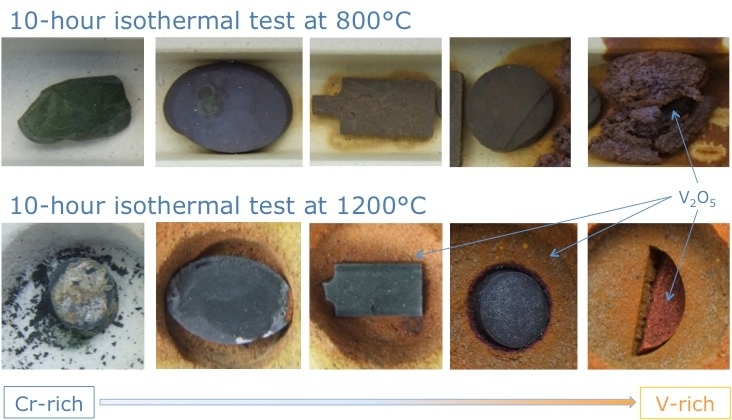
\includegraphics[width=22cm]{oxidation}
\caption{Photographs of the binary and ternary alloys after 1-hour exposures at 800\celsius\ and at 1200\celsius.   From left to right: Cr--Cr$_3$Si, ($\frac{3}{4}$Cr, $\frac{1}{4}$V)--($\frac{3}{4}$Cr, $\frac{1}{4}$V)$_3$Si, \ilovewill{山}, ($\frac{1}{4}$Cr, $\frac{3}{4}$V)--($\frac{1}{4}$Cr, $\frac{3}{4}$V)$_3$Si and V--V$_3$Si }\label{fig:oxidation}
\end{center}
\end{figure}
\end{landscape}
%


\section{Load-Partitioning Experiments}

In-situ neutron experiments were performed to determine the load-partitioning behaviour of the two phases present in X--X$_3$Si eutectics.  Specimens were subject to high-temperature compression-creep in experiments performed on the ENGIN-X beamline, at the ISIS pulsed neutron facility, Rutherford Appleton Laboratory, U.K..  

In diffraction, Bragg's law is used: 

\hspace{5cm}		$\lambda$ = 􏰄 2d$_{hkl}$sin$\theta$

where l is the wavelength, d$_{hkl}$ is the lattice plane spacing and $\theta$ is the Bragg angle.  

The ENGIN-X beamline is dedicated to the accurate measurement of lattice parameters at a known location within a crystalline specimen.  Changes in spacing between the atomic lattice planes is detected from the changes in diffraction peak angles, and this can be translated to strain:

\hspace{5cm}	$\epsilon$ = -cot $\theta$ $\delta$$\theta$

A 'white', polychromatic neutron beam is used at ENGIN-X.  It has a neutron flight path of 50\metre. The time-of-flight (TOF) method is required to utilise this.  The choppers were set to allow 1 out of 2 pulses from the target to enter the diffractometer.  It has two banks of diffraction bank detectors positioned at $\pm$ 90\degree\ to the incident beam (Figure \ref{fig:enginxsetup}).  These banks measure time-resolved spectra with scattering vectors axially and transversely aligned with the loading axis.  Incidence slits and 4mm radial collimators were used to define a gauge volume of 4x4x4mm within the centre of each test specimen.  The loading axis is horizontal and positioned at 45\degree\ to the incident beam (Figure \ref{fig:enginxsetup}).  This set-up enables the measurement of lattice strains in axes that are parallel and perpendicular to applied load.  This characteristic was fully utilised in a diffraction experiment that quantified the degree of lattice misfit in the vertical and horizontal interfaces between $\gamma$ and $\gamma$'.  The Instron screw thread tensile stress-rig used for the experiment was mounted upon a high capacity translation and rotation stage.  A high-temperature mirror-furnace encapsulated the specimen-chamber to provide a high-temperature environment of up to 900\celsius\ comfortably, but was pushed to 1000\celsius\ under close supervision for this experiment.  A LOCOMETRIC precision specimen-mounting system is used to ensure reproducibility of specimen positioning.  Bespoke alumina platens were made to fit into the stress-rig grips to convert the tensile stress-rig to a compressive stress-rig.  Alumina is neutron transparent, and would not interfere with the experiment.  A Pt/Pt-Rh thermocouple was tied onto the each test specimen to monitor specimen temperature. 

In this experiment, it was hoped that load partitioning from the solid-solution to the harder silicide phase would be seen.  This would be seen as an increase in the elastic strain on silicide peaks as creep progressed.  All specimens were subject to constant applied stress versus time.  When each test specimen was fully loaded to the desired compression condition, a dwell-time of a minute was allocated to allow for specimen stress relaxation prior to the initiation of data acquisition. Each data-set of peak profiles could be collected over 15--20 minutes if no neutron beam instabilities were encountered.  Load and displacement outputs were acquired every few seconds.

Load-partitioning experiments have been successfully performed on other systems such as continous fibre composites ~\cite{withers98} and nickel-based superalloys ~\cite{coakley12, dye01}.  This is not a novel experimental set-up.


%
\begin{figure}[htbp]
\begin{center}
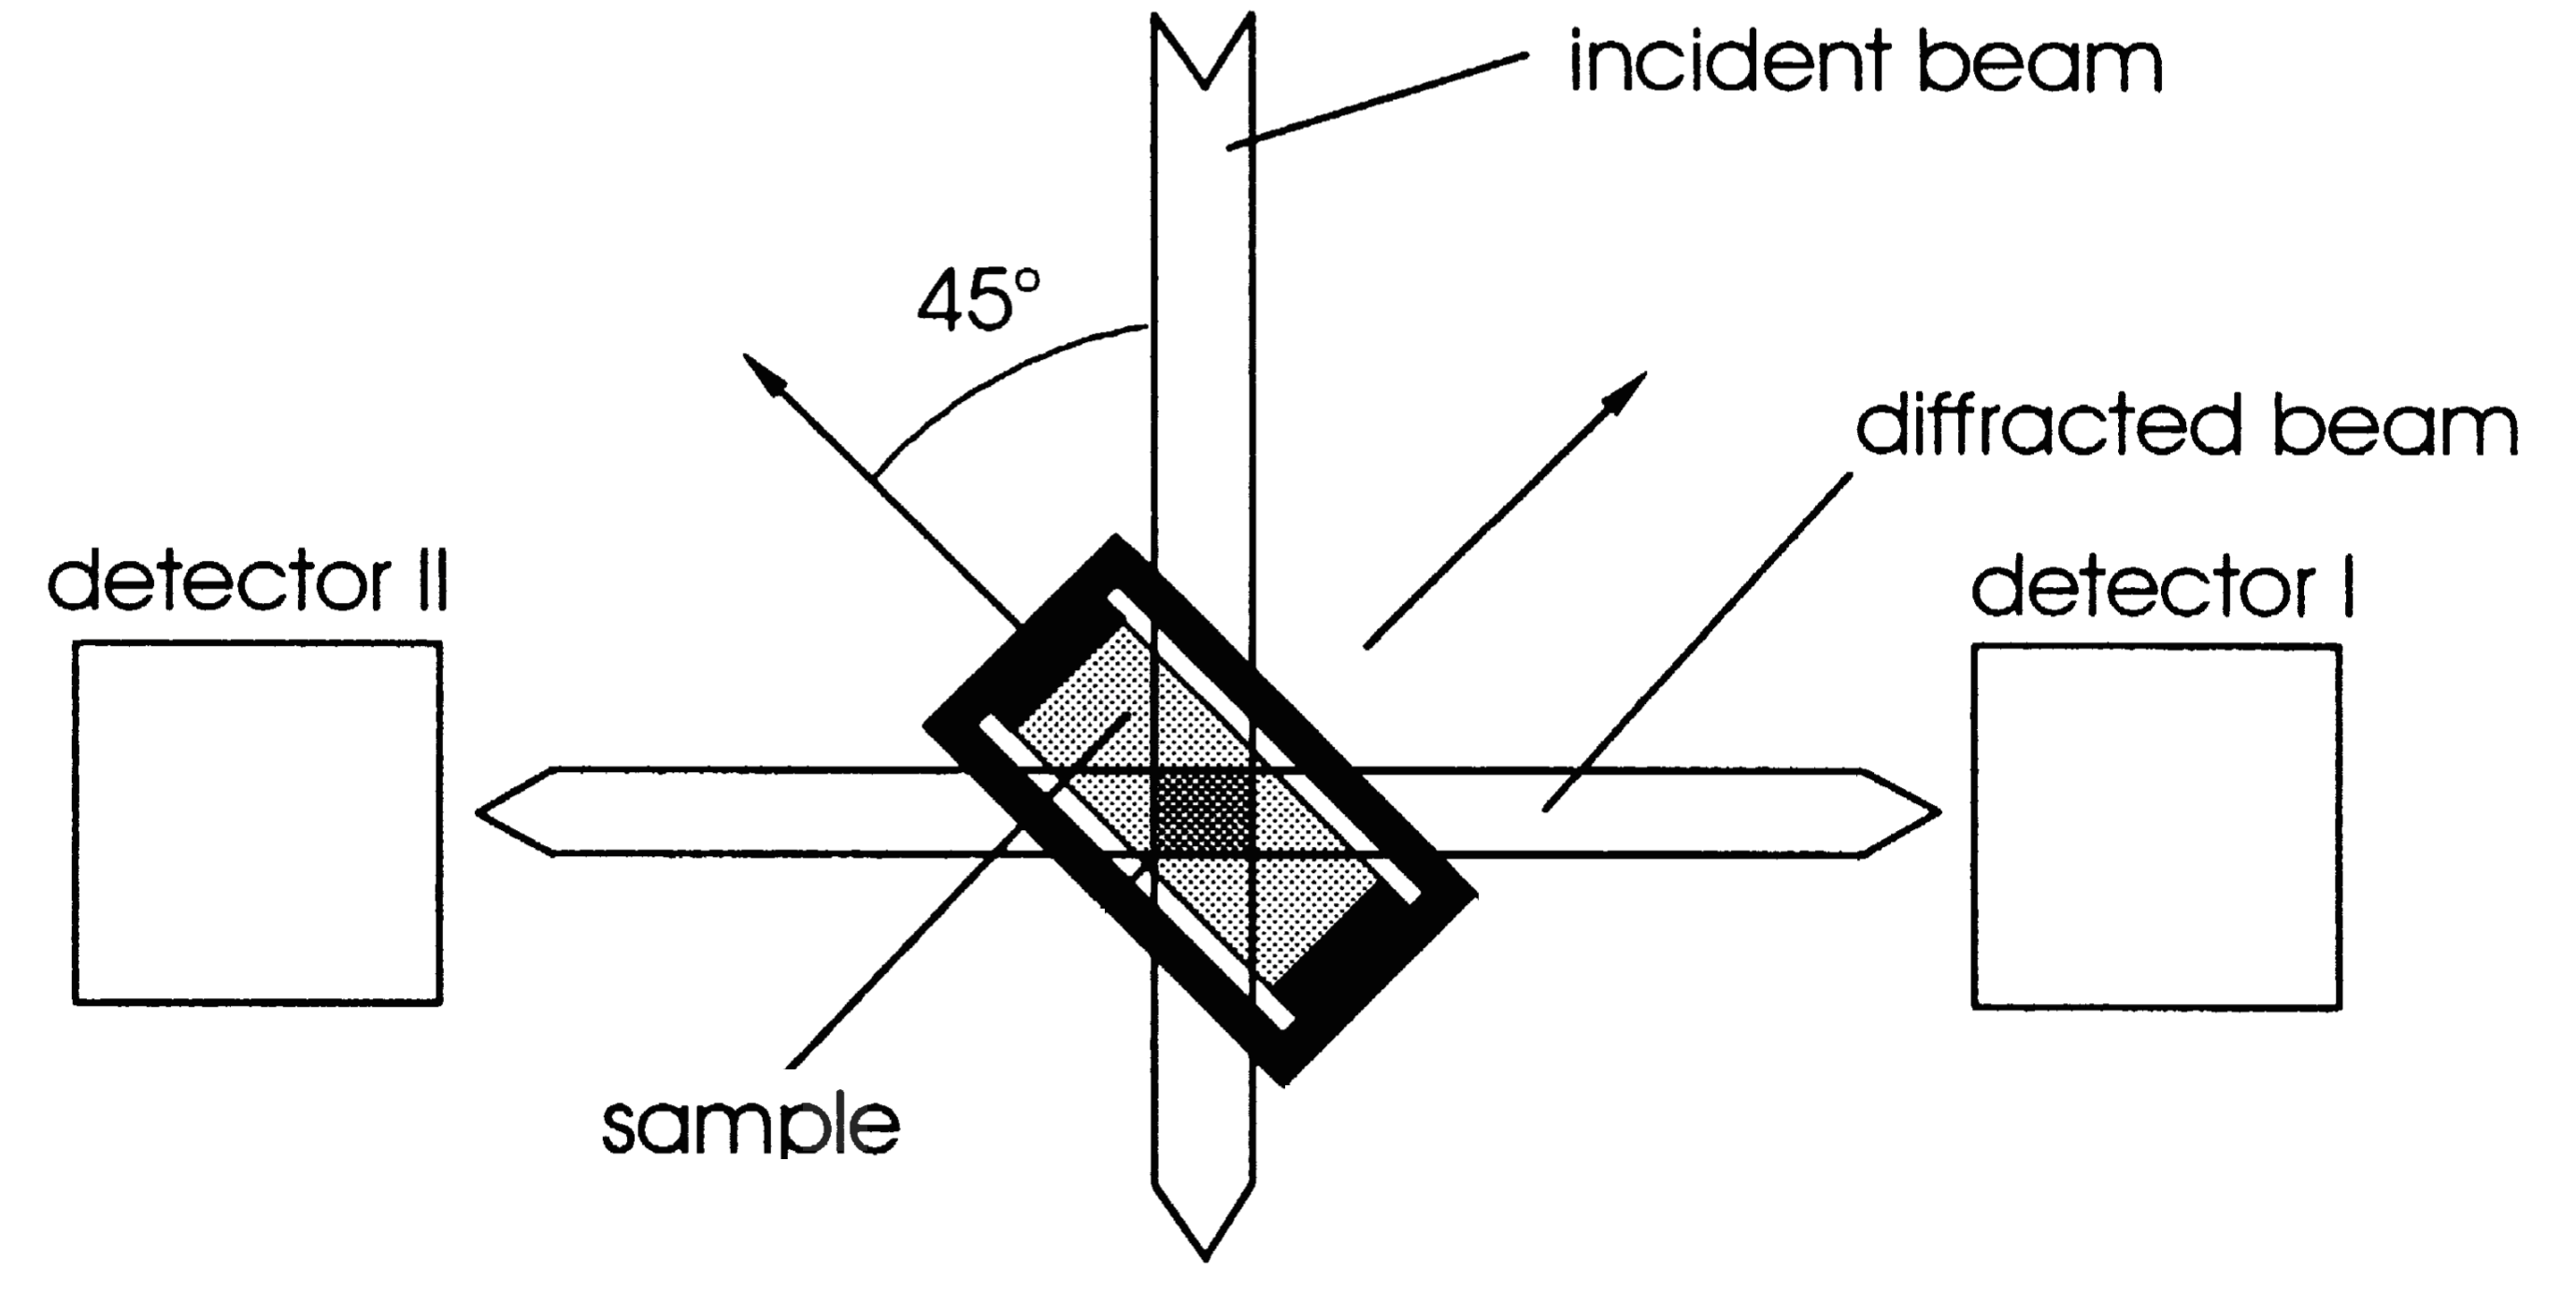
\includegraphics[width=10cm]{enginxsetup}
\caption{Schematic of experimental set-up at the Engin-X beamline.}\label{fig:enginxsetup}
\end{center}
\end{figure}
%

%

\begin{table}[htdp]
\begin{center}
\begin{tabular}{lcccc}
\hline
\hline
d ($\angstrom$)		&Cr		&Cr$_3$Si							&Time of Flight approximation (\micro\second)\\
\hline
2.27	&No peak	&200								&41768\\
2.04	&110		&210 (may be small)				&37536\\
1.45	&200		&310 (powdercell says small)		&26680\\
1.177	&211		&No peak							&21656.8\\
1.13	&No peak	&400								&20792 \\
1.02	&220		&420								&18768 \\
0.912	&310		&No peak							&16780.8 \\
\hline
\hline
\end{tabular}
\end{center}
\caption{Time of flight approximations for possible peaks, together with their corresponding d-spacings.}
\label{tab:tof}
\end{table}

The prediction of peaks was performed in the software program called Powdercell.  Observable peaks, their corresponding d-spacings and time of flight approximations have been put into Table \ref{tab:tof}.  From this, the time of flight (TOF) range for this experiment is between 16780 and 41768\micro\second.  Peaks that have major contributions from both phases may not show clear trends during load-partitioning.  One such peak has a d-spacing of 1.02$\angstrom$ with contributions from Cr (220) and Cr$_3$Si (420).  The peaks that have contribution from one phase have a higher probability of exhibiting peak shifts stemming from the partioning of load.  The Cr$_3$Si (200) peak, and the Cr (310) peak are ideal peaks to examine.  

Test specimens used were DS processed cylinders measuring 8\milli\metre\ in diameter and 18\milli\metre\ tall.  Isotropic specimens would produce more peaks for ease of fitting. PM manufactured material had the highest degree of isotropy in this project.  The V--V$_3$Si specimens were cut from PM manufactured material.  For other alloys, such ingots did not have structural integrity and were not used.    

Vanadium is transparent to neutrons.  Alloys with high V content, such as V--V$_3$Si and \ilovewill{山}, did not produce sufficient peak intensities for robust fits.  

EX-SBA, a bespoke peak-fitting program written in Open Genie programming language, was developed at ISIS to analyse neutron diffraction spectra measured at ENGIN-X.  This was used to fit the peak profiles acquired in this experiment, one peak at a time.

\subsection{Results}
 
It was hoped that strain-partitioning in the two phases could be seen in the elastic regime, and that an evolution or divergence in strain-partitioning behaviour would be observed once the specimens were in the plastic regime.

Elastic strain of characteristic peaks of the BCC solid-solution and the A15 X$_3$Si phase were measured as a function of cross-head displacement.  Cross-head displacement was set to occur at a constant rate.  Cr--C$_3$Si experienced visible creep at 910\celsius/200\mega\pascal\ (Figure \ref{fig:enginxcr910C200MPa}).
The shifts in peak versus times can be seen in Figure \ref{fig:enginxcr910Cstrain}. There is a downward, compressive trend in elastic strain for all peaks.  Both phases experienced the same degree of elastic strain.  Partitioning of load was not seen.  Cr--C$_3$Si experienced substantial deformation when subjected to 1000\celsius/200\mega\pascal\ (Figures \ref{fig:enginxcr1000C200MPa} and \ref{fig:enginxcr1000Cstrain}).  When in operation, the stress-rig would have a slight, sinusoidal fluctuation in stress, with a period of 20 minutes.  As mentioned in the high-temperature compression-testing section, the cause of this is unknown.

A PM processed \ilovewill{山}Ta specimen shattered when load was introduced at 900\celsius.  Pre-existing flaws must have diminished its integrity.  DS manufactured \ilovewill{山}Ta did not experience substantial creep deformation, except during the last 30 minutes when it was subjected to 910\celsius/308MPa (Figure \ref{fig:enginxsanta910C308MPa}).  The corresponding peak shifts in Figure \ref{fig:santa910C308MPastrain} seem to display noise.  The (211) peak shift for Cr (purple line) and the (400) peak shift for Cr$_3$Si (turquoise line) do not show any trends when noise is disregarded.

When DS manufactured \ilovewill{山}Ta was subjected to 1000\celsius/308MPa, creep was observed (Figure \ref{fig:enginxsanta1000C200MPa}).  This was unaccompanied by clear evidence of load partitioning, as seen in the plot of elastic strain versus time (Figure \ref{fig:enginxsanta1000C200MPastrain}).

%
\begin{figure}[H]
\begin{center}
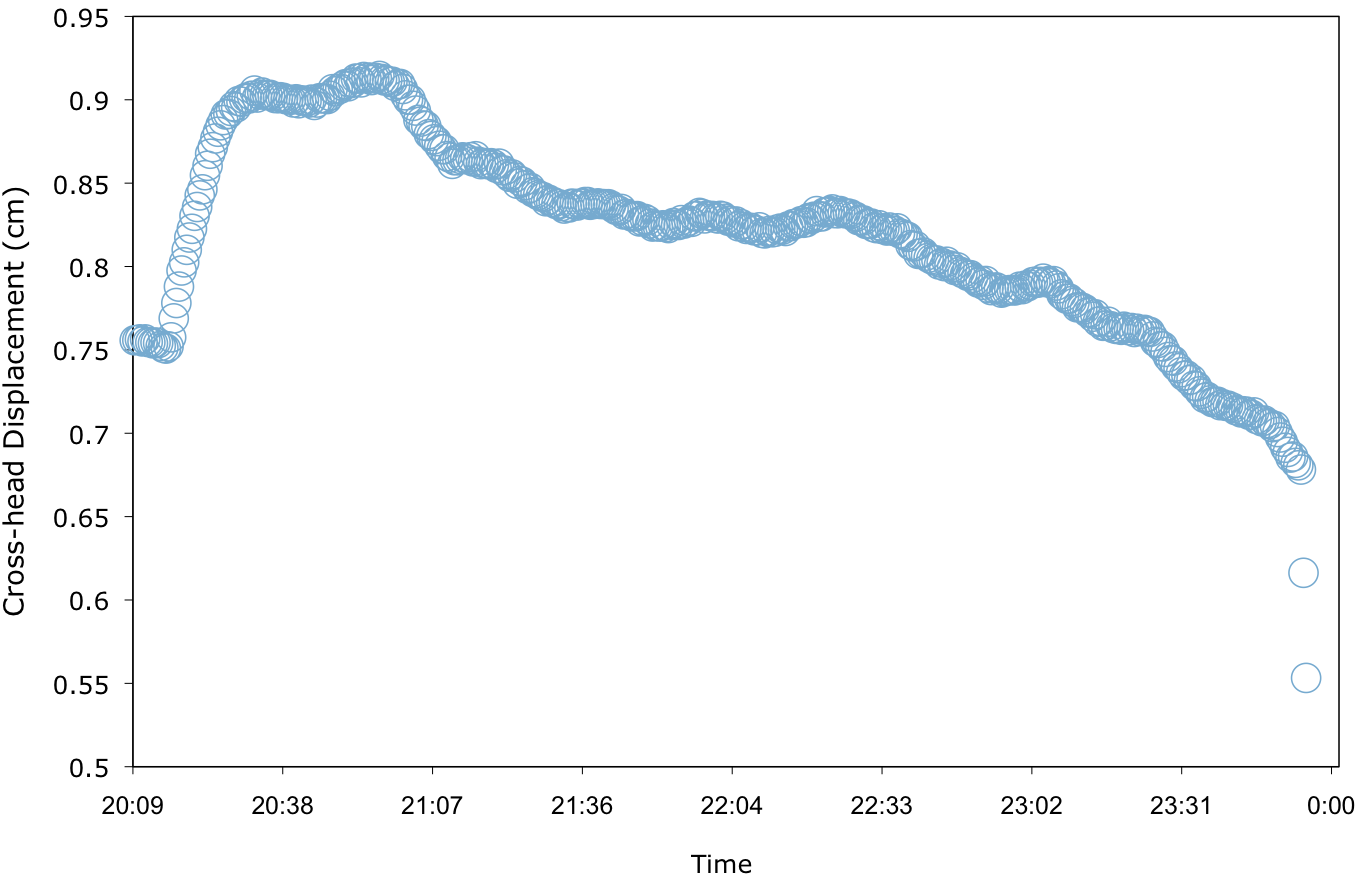
\includegraphics[width=14cm]{enginxcr910C200MPa}
\vspace{-2mm}
\caption{Plot of cross-head displacement vs time for DS manufactured Cr--Cr$_3$Si at 910\celsius/ 200MPa.}\label{fig:enginxcr910C200MPa}
\end{center}
\end{figure}  
%
%
\begin{figure}[H]
\begin{center}
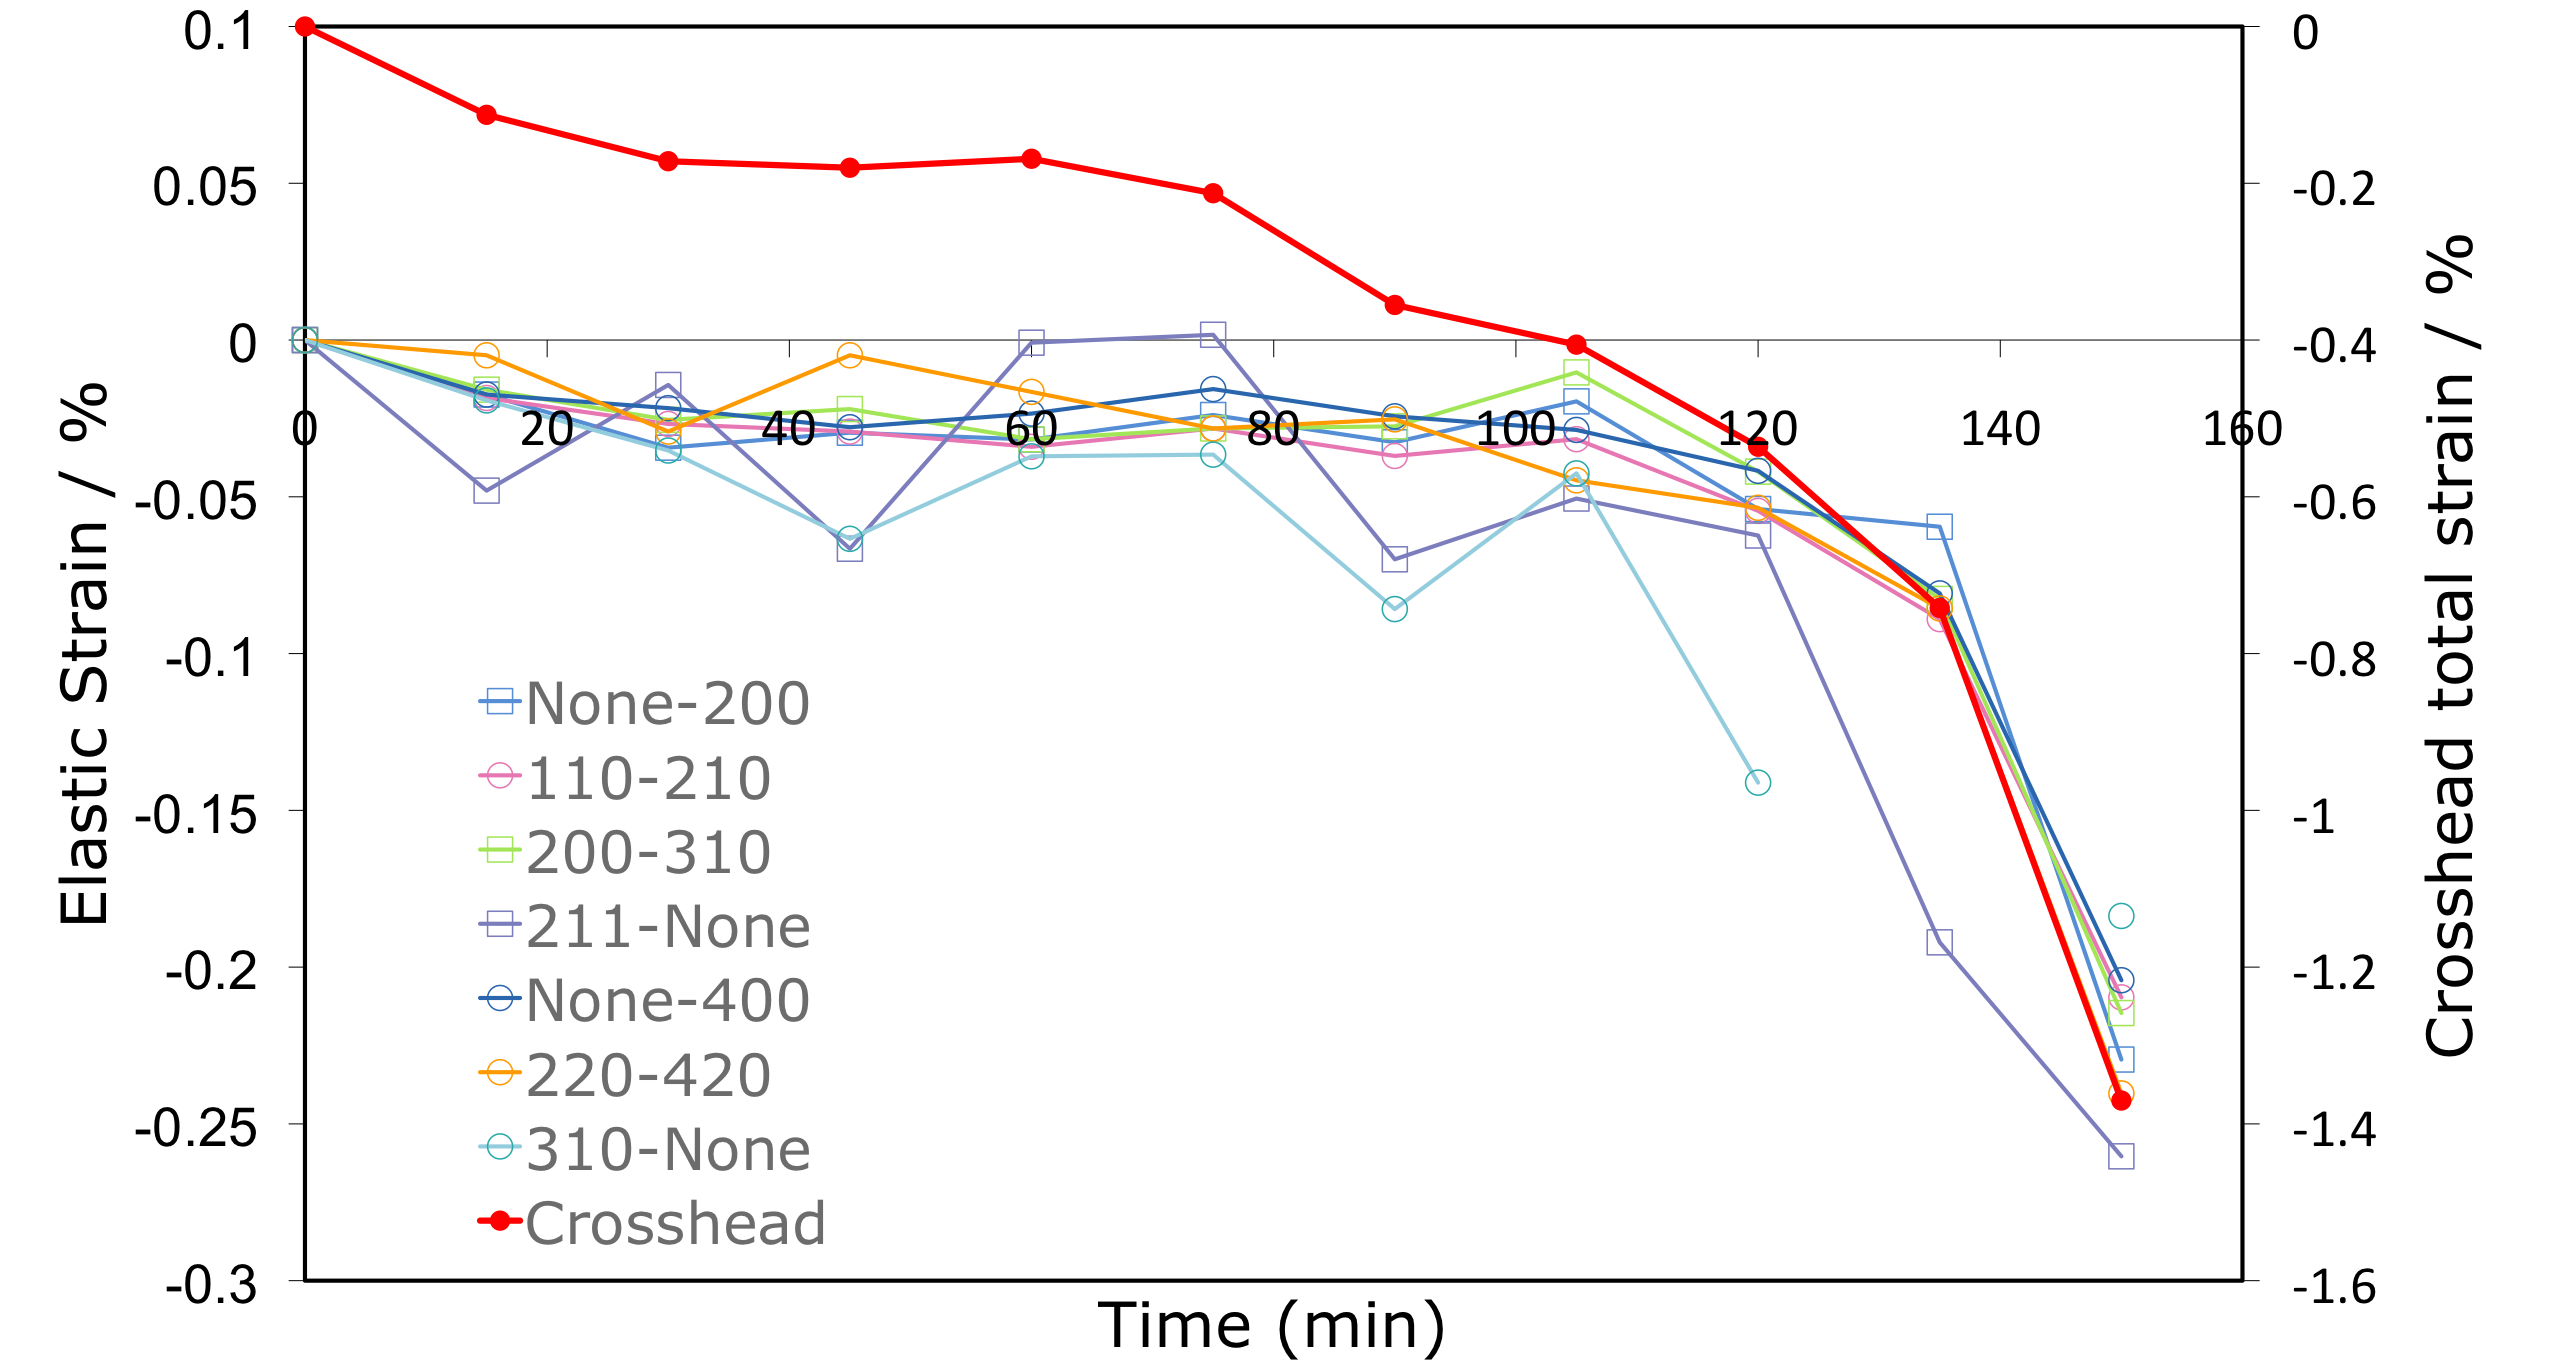
\includegraphics[width=16cm]{enginxcr910C200MPastrain}
\vspace{-2mm}
\caption{Plot of cross-head displacement, strain and peak shifts vs time for DS manufactured Cr--Cr$_3$Si at 910\celsius/ 200MPa.}\label{fig:enginxcr910Cstrain}
\end{center}
\end{figure}  
%
%
\begin{figure}[H]
\begin{center}
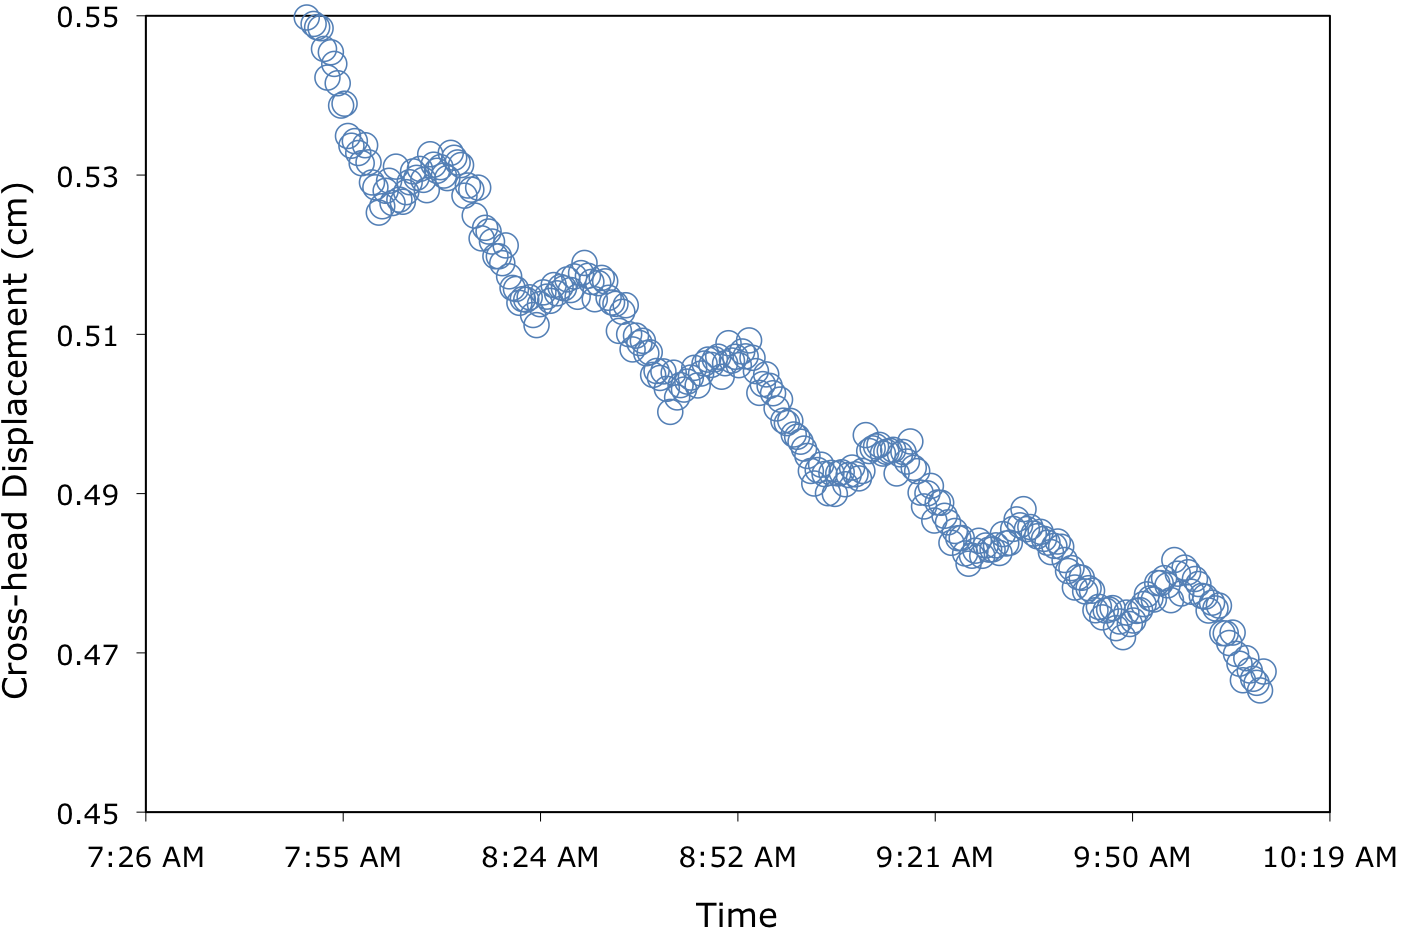
\includegraphics[width=12cm]{enginxcr1000C200MPa}
\vspace{-2mm}
\caption{Plot of cross-head displacement vs time for DS manufactured Cr--Cr$_3$Si at 1000\celsius/ 200MPa.}\label{fig:enginxcr1000C200MPa}
\end{center}
\end{figure}  
%
%
\begin{figure}[H]
\begin{center}
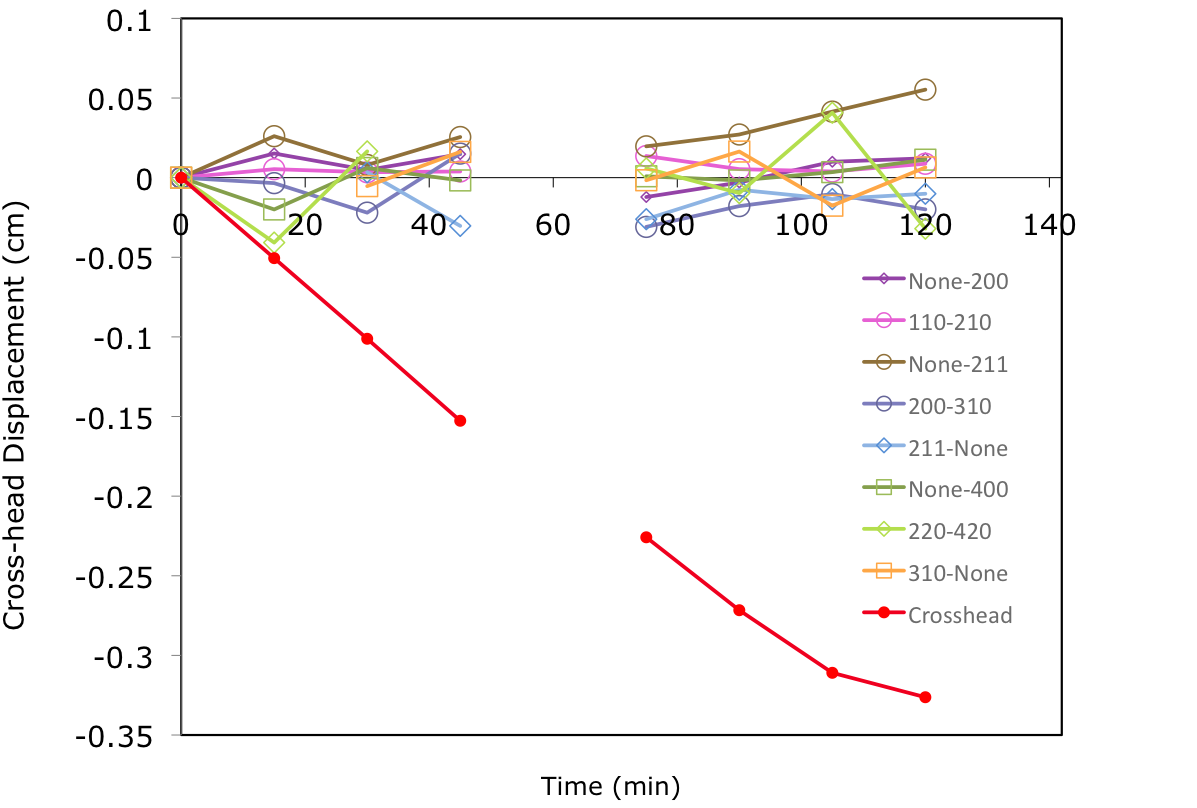
\includegraphics[width=15cm]{enginxcr1000C200MPastrain}
\vspace{-2mm}
\caption{Plot of cross-head displacement, strain and peak shifts vs time for DS manufactured Cr--Cr$_3$Si at 1000\celsius/ 200MPa.}\label{fig:enginxcr1000Cstrain}
\end{center}
\end{figure}  
%
%
\begin{figure}[H]
\begin{center}
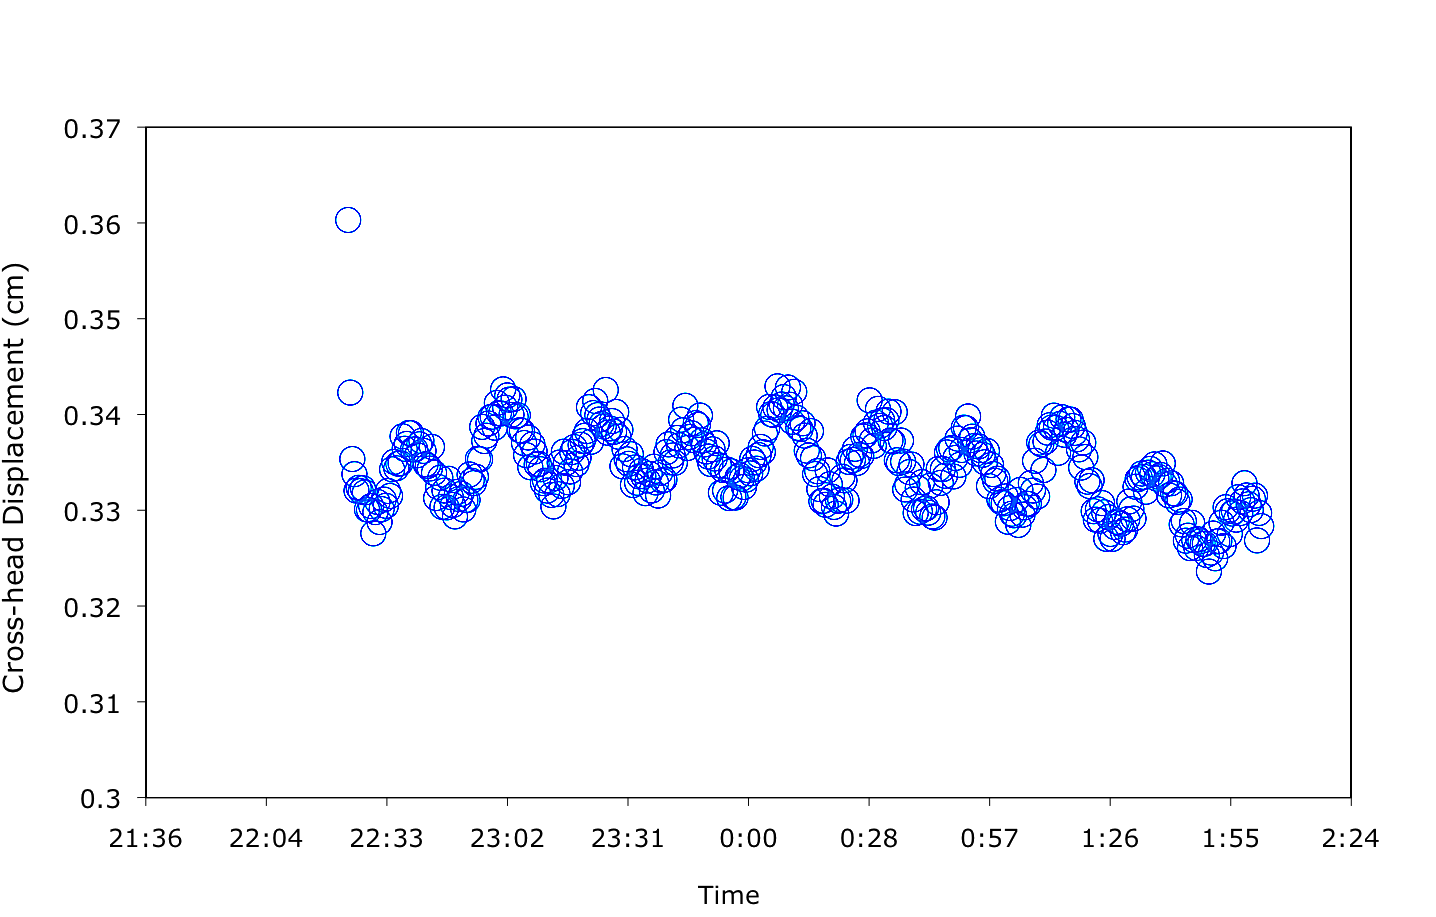
\includegraphics[width=14cm]{enginxsanta910C308MPa}
\vspace{-2mm}
\caption{Plot of cross-head displacement vs time for \ilovewill{山}Ta at 910\celsius/ 308MPa.}\label{fig:enginxsanta910C308MPa}
\end{center}
\end{figure}  
%
%
\begin{figure}[H]
\begin{center}
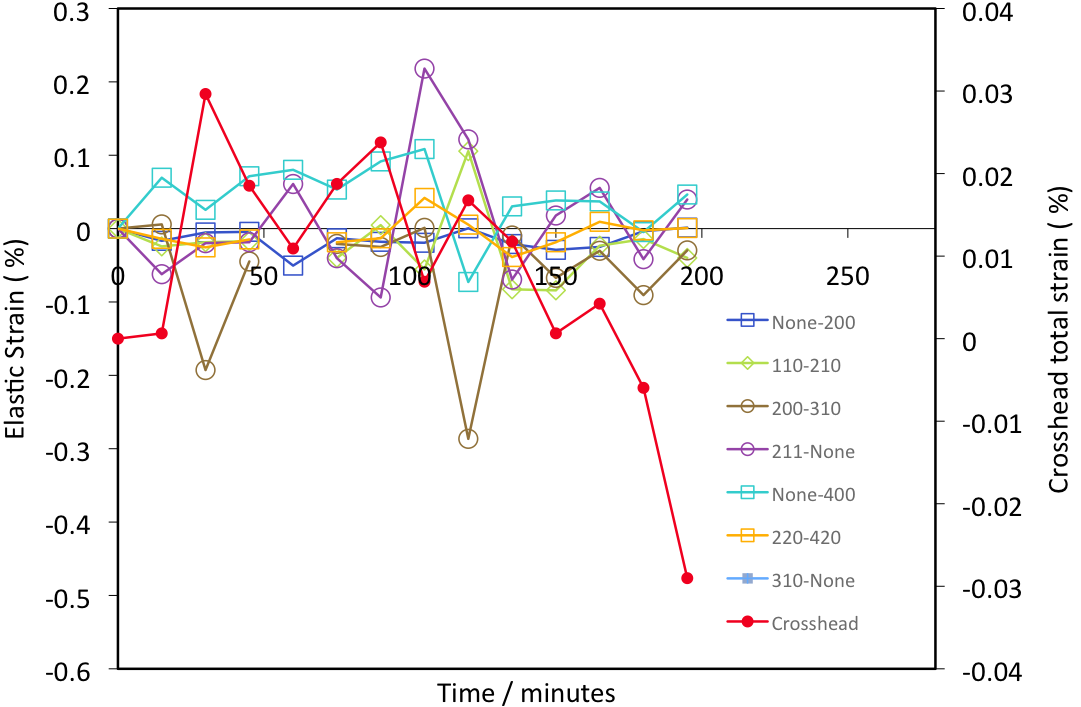
\includegraphics[width=16cm]{enginxsanta910C308MPastrain}
\vspace{-2mm}
\caption{Plot of cross-head displacement and peak shifts vs. time for \ilovewill{山}Ta at 910\celsius/ 308MPa.}\label{fig:santa910C308MPastrain}
\end{center}
\end{figure}  
%
%
\begin{figure}[H]
\begin{center}
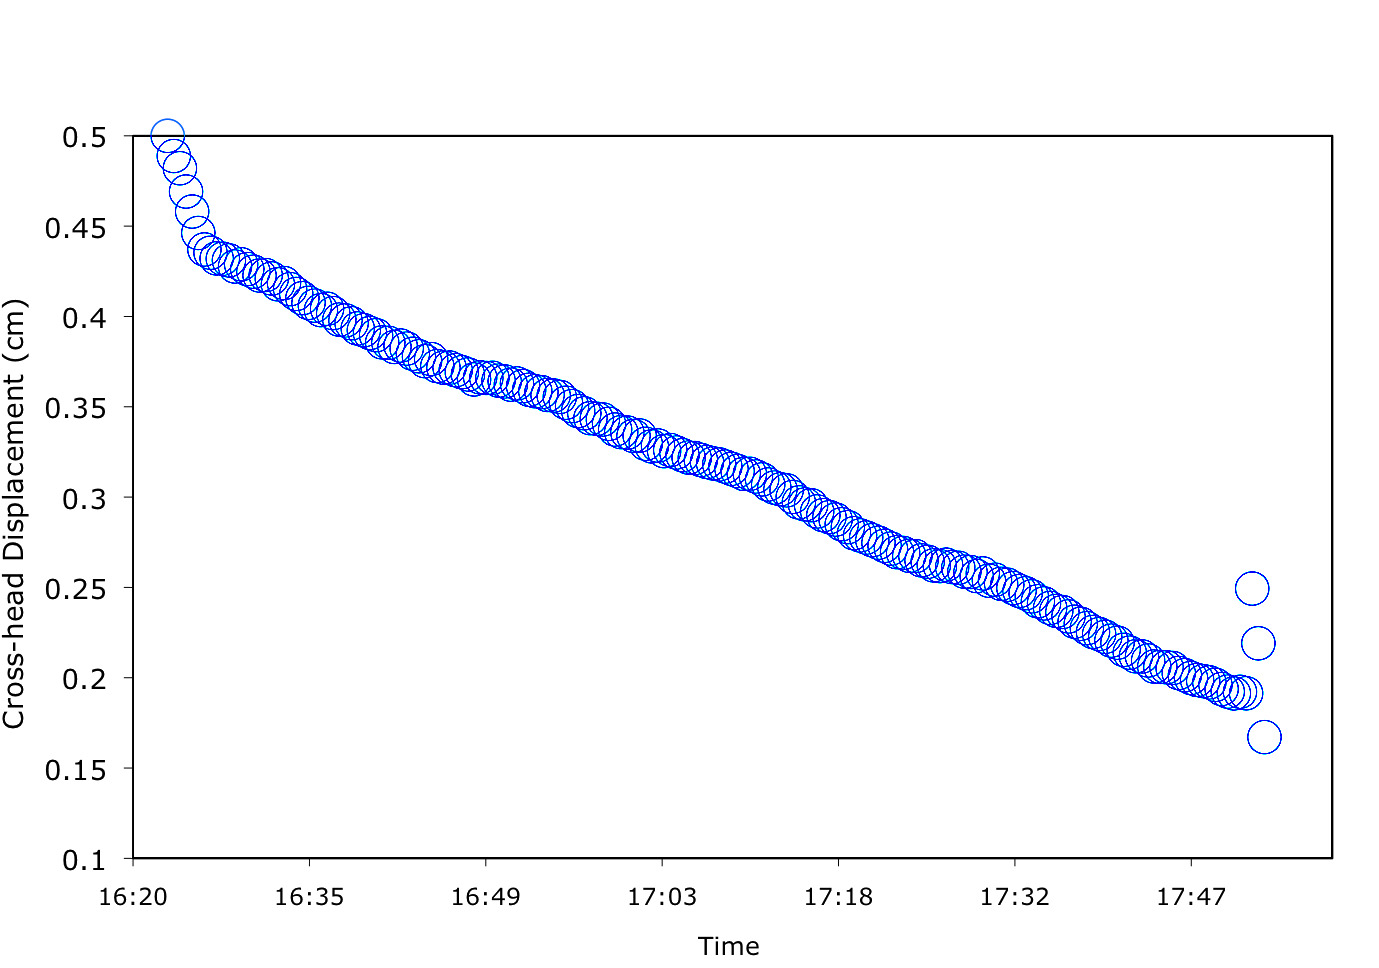
\includegraphics[width=11.5cm]{enginxsanta1000C200MPa}
\vspace{-2mm}
\caption{Plot of cross-head displacement vs time for \ilovewill{山}Ta at 1000\celsius/ 200MPa.}\label{fig:enginxsanta1000C200MPa}
\end{center}
\end{figure}  
%
%
\begin{figure}[H]
\begin{center}
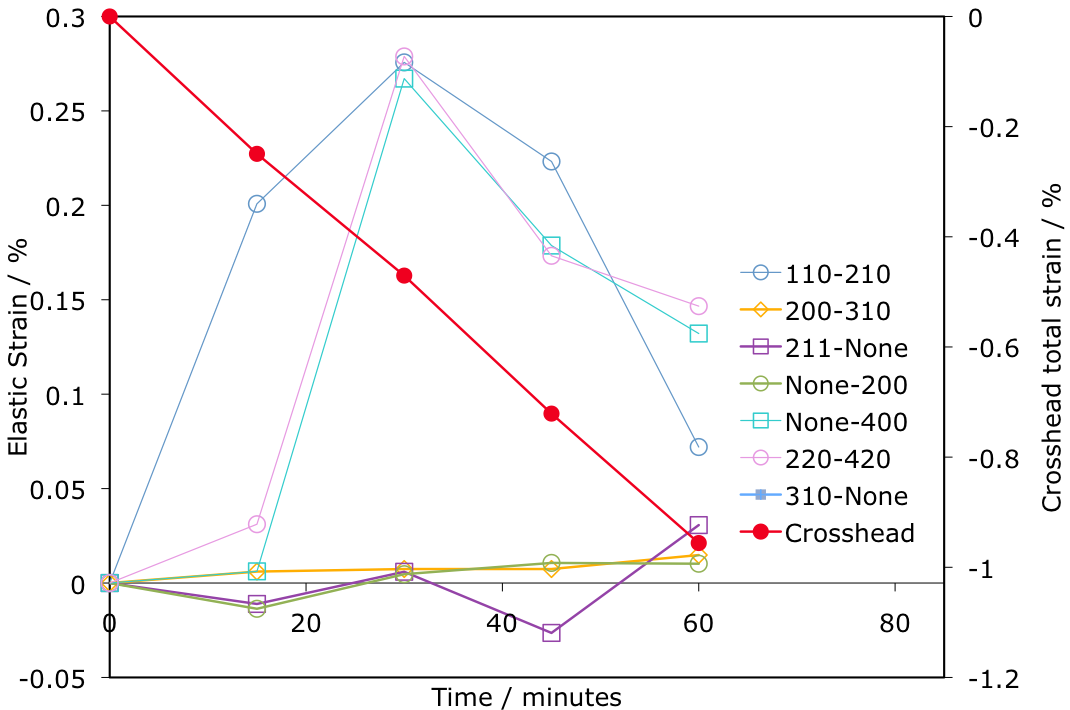
\includegraphics[width=16cm]{enginxsanta1000C200MPastrain}
\vspace{-2mm}
\caption{Plot of elastic strain and peak shifts vs. time for \ilovewill{山}Ta at 1000\celsius/ 200MPa.}\label{fig:enginxsanta1000C200MPastrain}
\end{center}
\end{figure}  
%

There is only one slightly plausible piece of evidence of load partitioning.  Slight deviation from linearity was seen in the (211) peak at the end of the experiment for the intermetallic phase in the Cr--Cr$_3$Si specimen subjected to 1000\celsius/200\mega\pascal\ (Figure \ref{fig:enginxcr1000Cstrain}).  This data is represented by an olive line that seemed to increase in strain near the end of the experiment.  This deviation from linearity could be considered to be of similar magnitude as experimental uncertainty.  If this were to be the case, then there were no visible trends, and no conclusions could be drawn.

A neutron synchrotron is the best place to conduct such experiments.  Rapid data acquisition allows for many data points to be collected.  Phenomena that evolve over a short time period can be captured.

Withers subjected an incoherent Ti-SiC composite to increasing stress versus time in an experiment that was performed on the L3 spectrometer of the NRU reactor in Chalk River, Canada ~\cite{withers98}.  In this experiment, the acquisition times are very long due to a weak source.  If the loading condition had been constant applied stress, load partitioning may occur on a shorter timescale than can be captured by the diffractometer.  Load partitioning was successfully observed in this experiment (Figure \ref{fig:withers}).  The peaks from Ti (Figure \ref{fig:withers}a-c) shifted linearly between 0--700\mega\pascal, and deviated from linearity at a lattice strain of 0.0035--0.004 because Ti could not take up any more load. The peak for the harder SiC phase deviated in the opposite direction when Ti began to deform plastically  (Figure \ref{fig:withers}d).

%
\begin{figure}[H]
\begin{center}
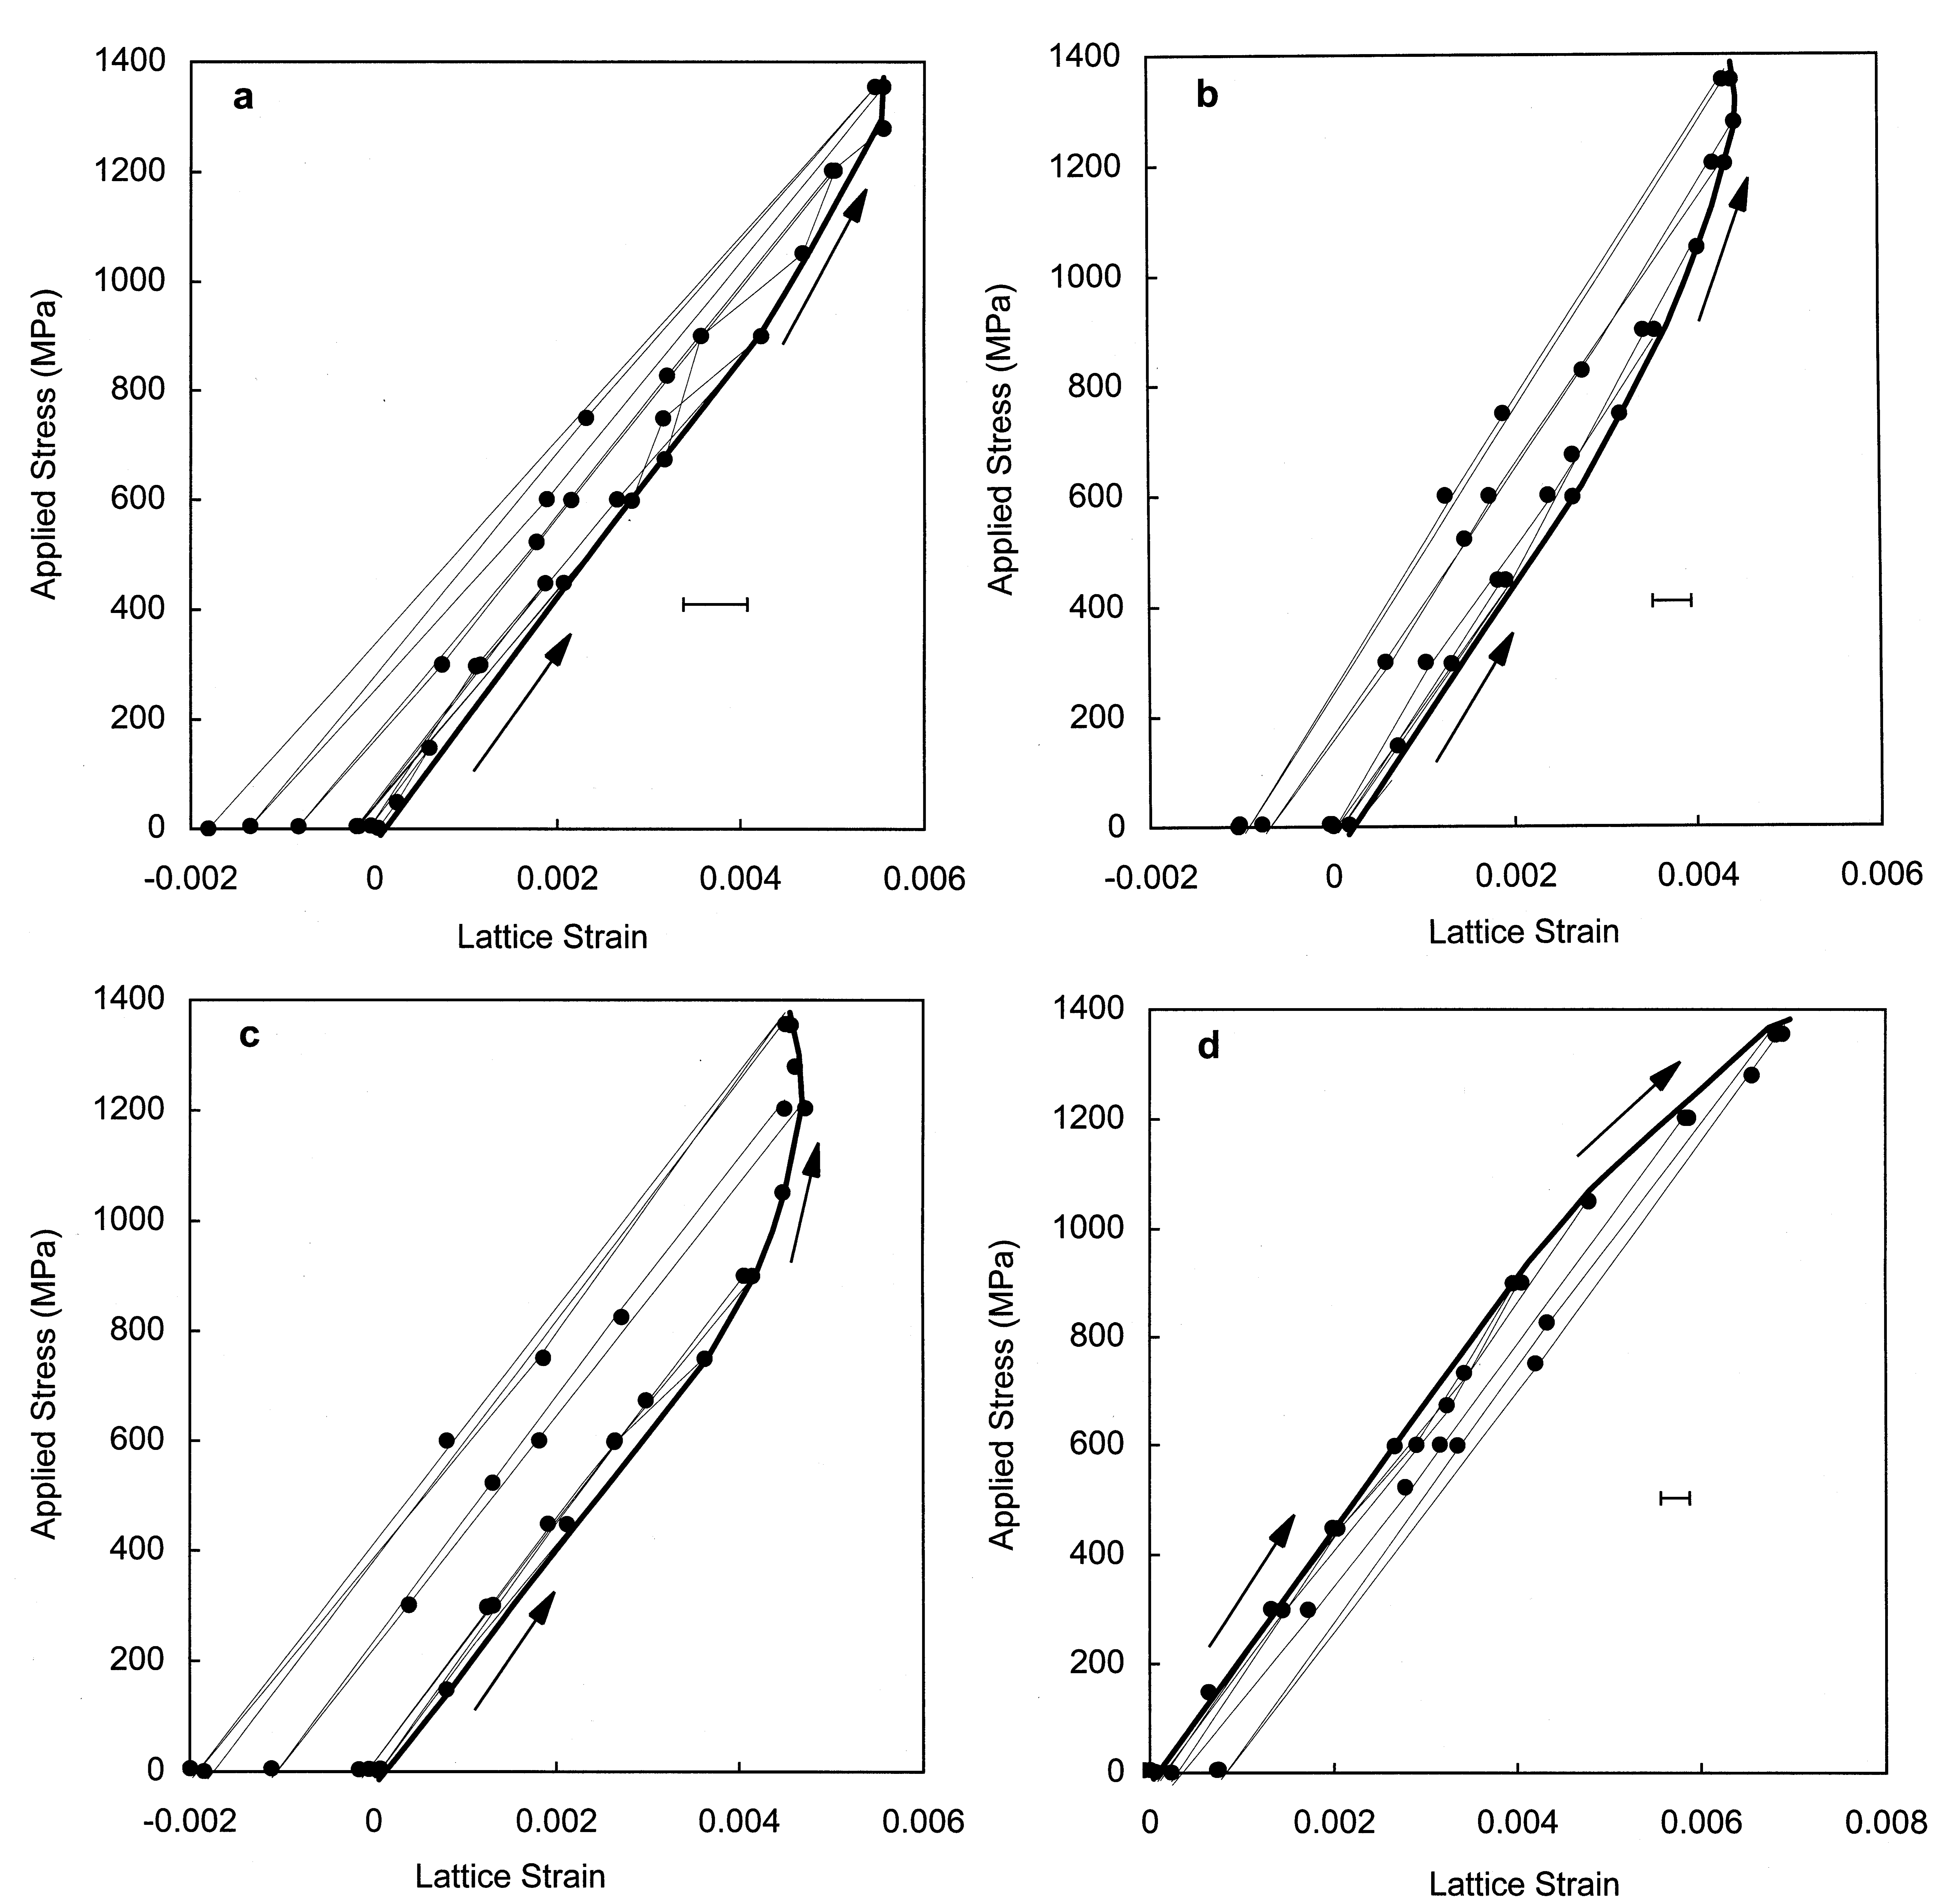
\includegraphics[width=16cm]{withers}
\vspace{-2mm}
\caption{The applied stress/lattice strain response for (a) the Ti􏰊(10$\bar{1}$0􏰋), (b) the Ti(0002), (c) the Ti(􏰊1011􏰋) and (d) the SiC(220) reflections.  The thin lines delineate the unloading/reloading stages of the cycle ~\cite{withers98}.}\label{fig:withers}
\end{center}
\end{figure}  
%

Coakley et. al subjected superalloy specimens under high-temperature creep.  The constant loading condition of this experiment allowed for the acquisition of good data ~\cite{coakley12}.  Under such conditions, the extent of load partitioning is significantly less than in experiments with increasing stress versus time. 

%
\begin{figure}[H]
\begin{center}
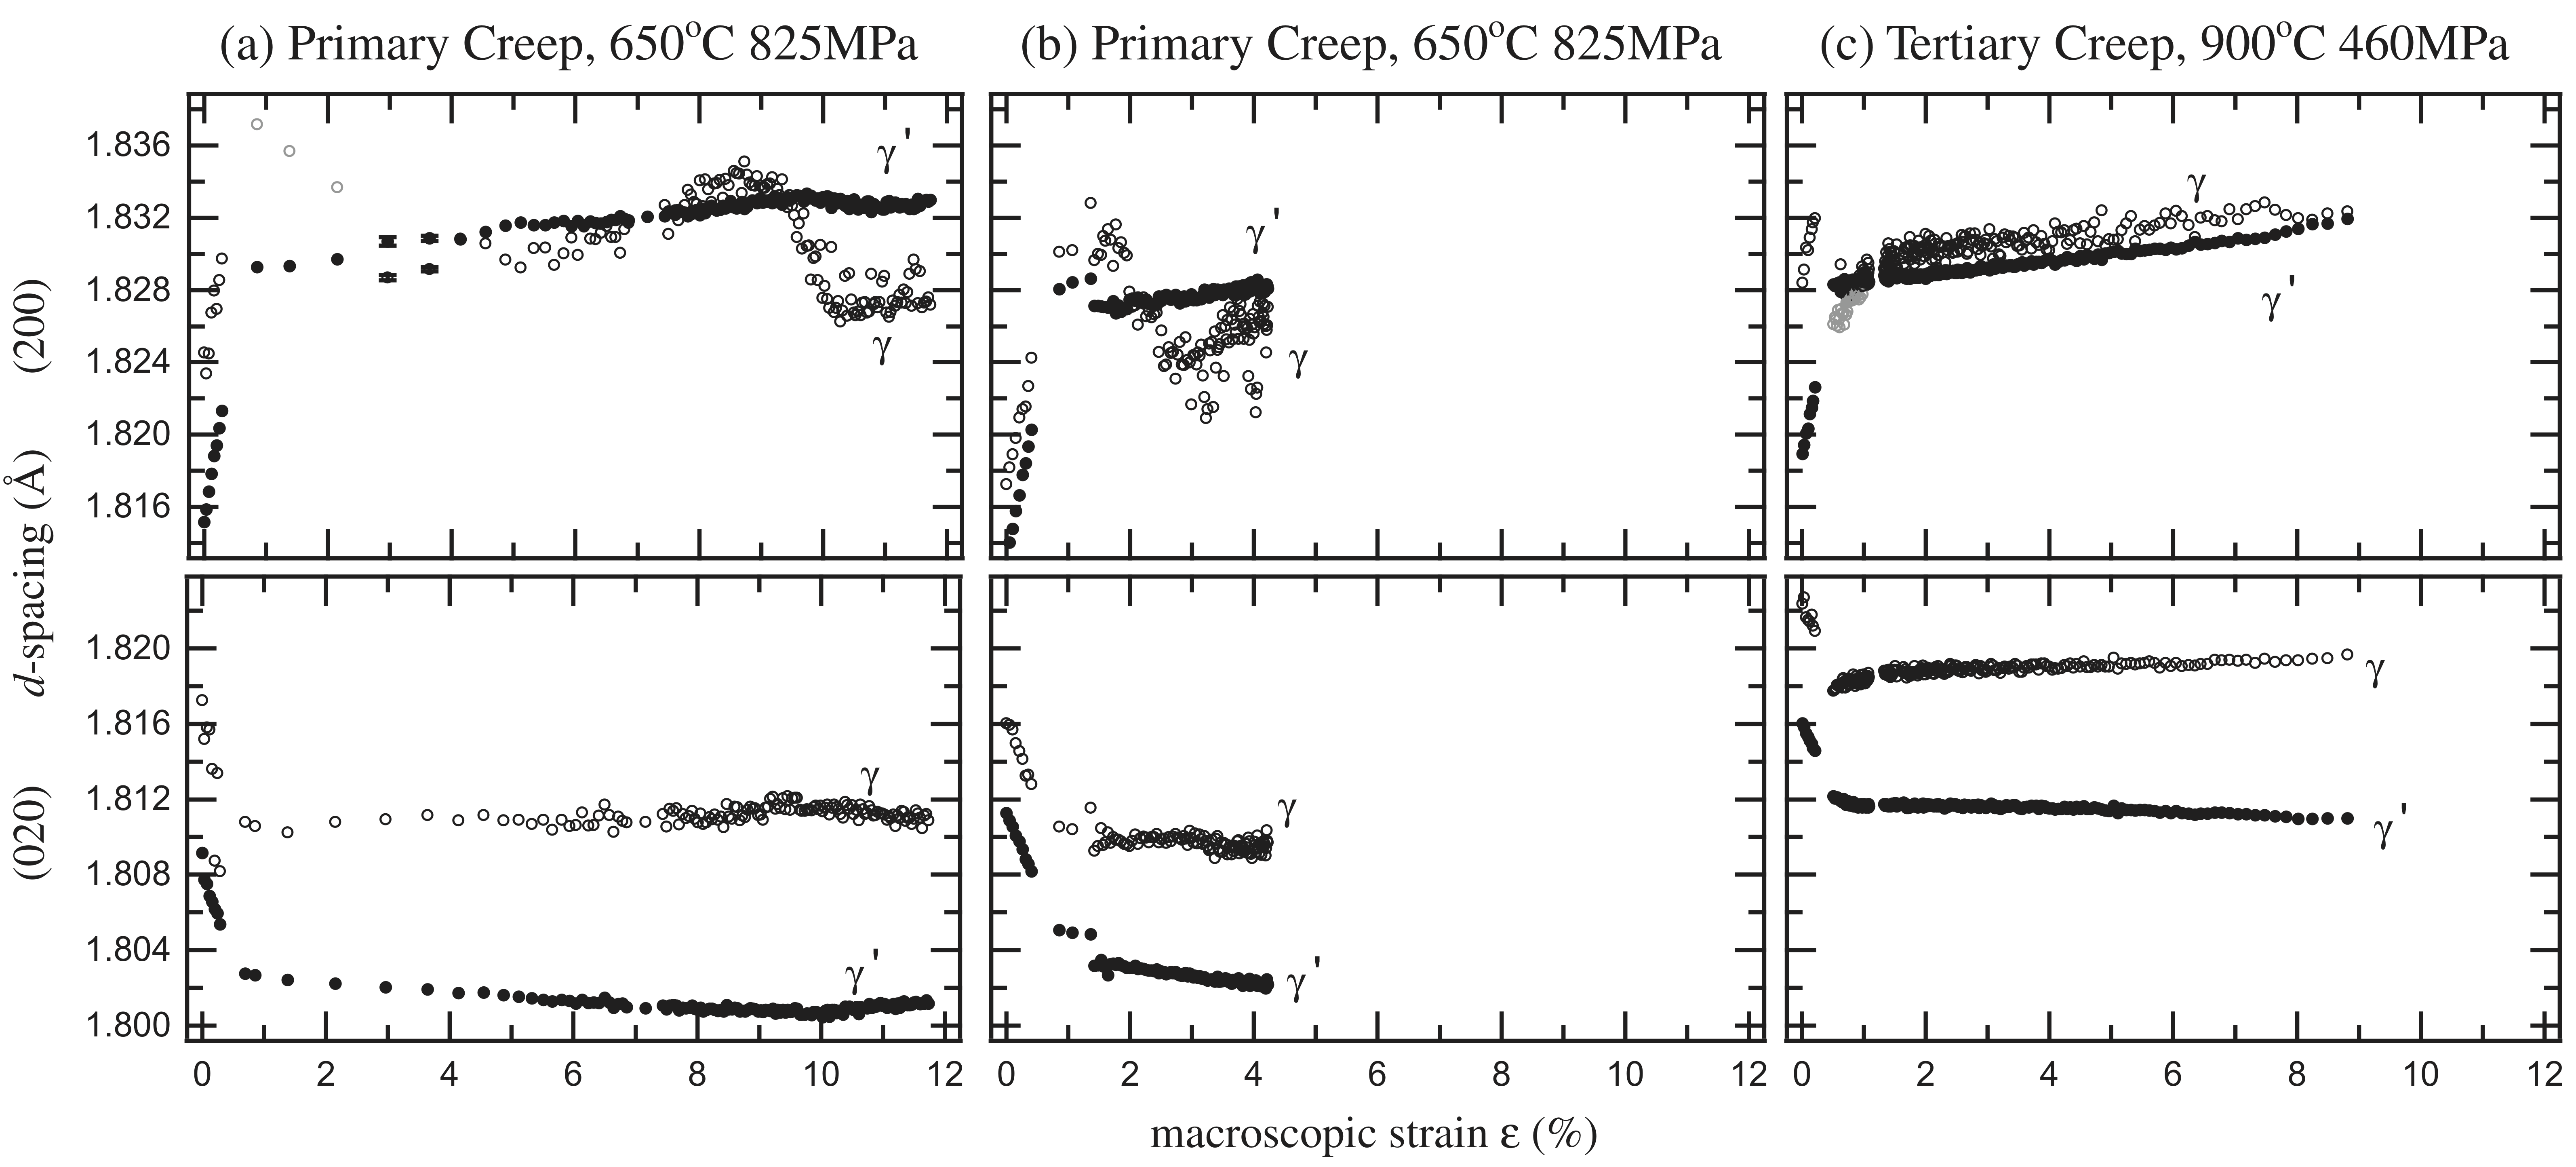
\includegraphics[width=16.5cm]{coakley}
\vspace{-2mm}
\caption{The d-spacing response during elastic loading and creep under two different operating conditions: top row, longitudinal (200) data, bottom row, transverse (020) data. $\gamma$ d-spacing data from peaks which proved difficult to fit accurately are highlighted in grey in (a) and (c) ~\cite{coakley12}.}\label{fig:coakley}
\end{center}
\end{figure}  
%

The expectation of seeing a degree of partitioning of load to the silicide phase was a reasonable one.  Nonetheless, despite repeated efforts to quantify the load partitioning between the solid-solution and the intermetallic X$_3$Si phase, our results merely show data scatter, and no visible trends.  No useful conclusions can be drawn.

